\documentclass[11pt,a4paper]{article}
\usepackage{fontspec}
\defaultfontfeatures{Mapping=tex-text}
\usepackage{xunicode}
\usepackage{xltxtra}
\usepackage{unicode-math}
%\setmainfont{Libertinus Serif}
%\setmathfont{Libertinus Math}
\usepackage[libertinus]{fontsetup}
\usepackage{polyglossia}
\setdefaultlanguage{english}
%\usepackage{amsmath}
%\usepackage{amsfonts}
%\usepackage{amssymb}
\usepackage{graphicx}
\usepackage[left=30mm,right=30mm,top=20mm,bottom=20mm]{geometry}
\usepackage[bookmarks=true,
            pdfencoding=unicode,
            allcolors=black,
            colorlinks=true,
            breaklinks=true]{hyperref}
\usepackage{caption}
\usepackage{subcaption}
\usepackage{siunitx}
\sisetup{output-decimal-marker = {.}, group-minimum-digits = 4, exponent-product = {\cdot}, inter-unit-product = {{\cdot}}, separate-uncertainty = true, arc-separator = \,, range-phrase=\:to\:, detect-all}
%\renewcommand{\baselinestretch}{1.25}

\begin{document}

%\begin{titlepage}
%	\begin{center}
%        \vspace*{2cm}
%        
%        \LARGE
%        Ipelet for Ipe software
%        
%        \vspace{0.1cm}
%        \Huge
%        \textbf{Axonometric projection}
%            
%        \vspace{0.5cm}
%        \Large
%            
%        Tomáš Drobil
%            
%        \vfill
%        \LARGE
%        
%        User manual% and documentation
%            
%        \vspace{12cm}
%            
%        %\includegraphics[width=0.4\textwidth]{university}
%            
%        \Large
%        Version 1.0\\
%        \today
%        \vspace{0.5cm}
%            
%    \end{center}
%\end{titlepage}

\begin{center}        
\vspace*{0.5cm}
\huge
The \textbf{Axonometric projections} ipelet

\vspace{0.25cm}

\large
\url{https://github.com/Tomas38/ipe-projections}

\vspace{0.25cm}

\Large
Tomáš Drobil

\large
2024-08-24 v1.0
\vspace{1cm}
\end{center}

\tableofcontents

\listoffigures

\newpage

\section*{About}
\addcontentsline{toc}{section}{About}

This ipelet makes drawing 3D schemes using proper axonometric projection very easy. The goal of the ipelet is to make possible creating such schemes in Ipe software in an intuitive way without need for other (more complicated) solutions like TikZ.

\section{Using the ipelet}

With this ipelet, you can transform objects (lines, rectangles, circles and more) into their axonometric projection. You can transform objects into $xy$, $xz$ or $yz$ plane, or any other plane defined by rotation one of these three planes, see Fig.~\ref{fig:ipe_access_ipelet}. It might be useful to use shortcuts when doing the projections. How the functions work should be clear from Fig.~\ref{fig:easy_explained}.

\begin{figure}[bh]
\begin{center}
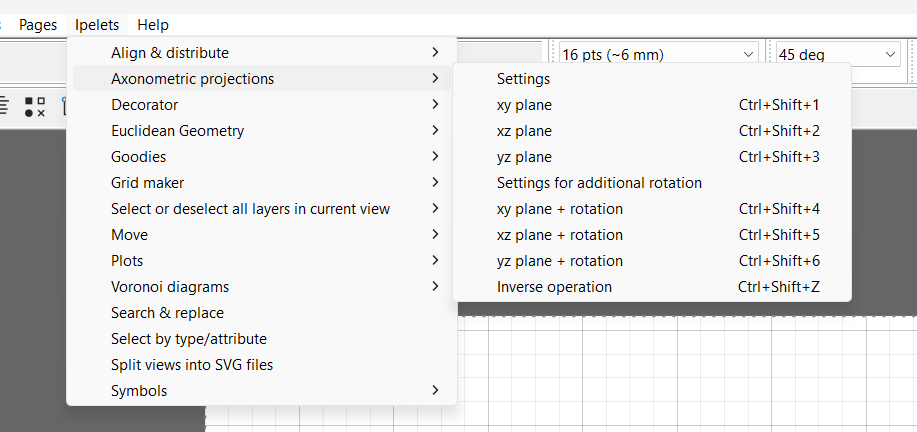
\includegraphics[scale=0.7]{png/main_menu.png}
\caption{How to access Axonometric projections ipelet fuctions and settings.}
\label{fig:ipe_access_ipelet}
\end{center}
\end{figure}

\begin{figure}[bh]
\centering
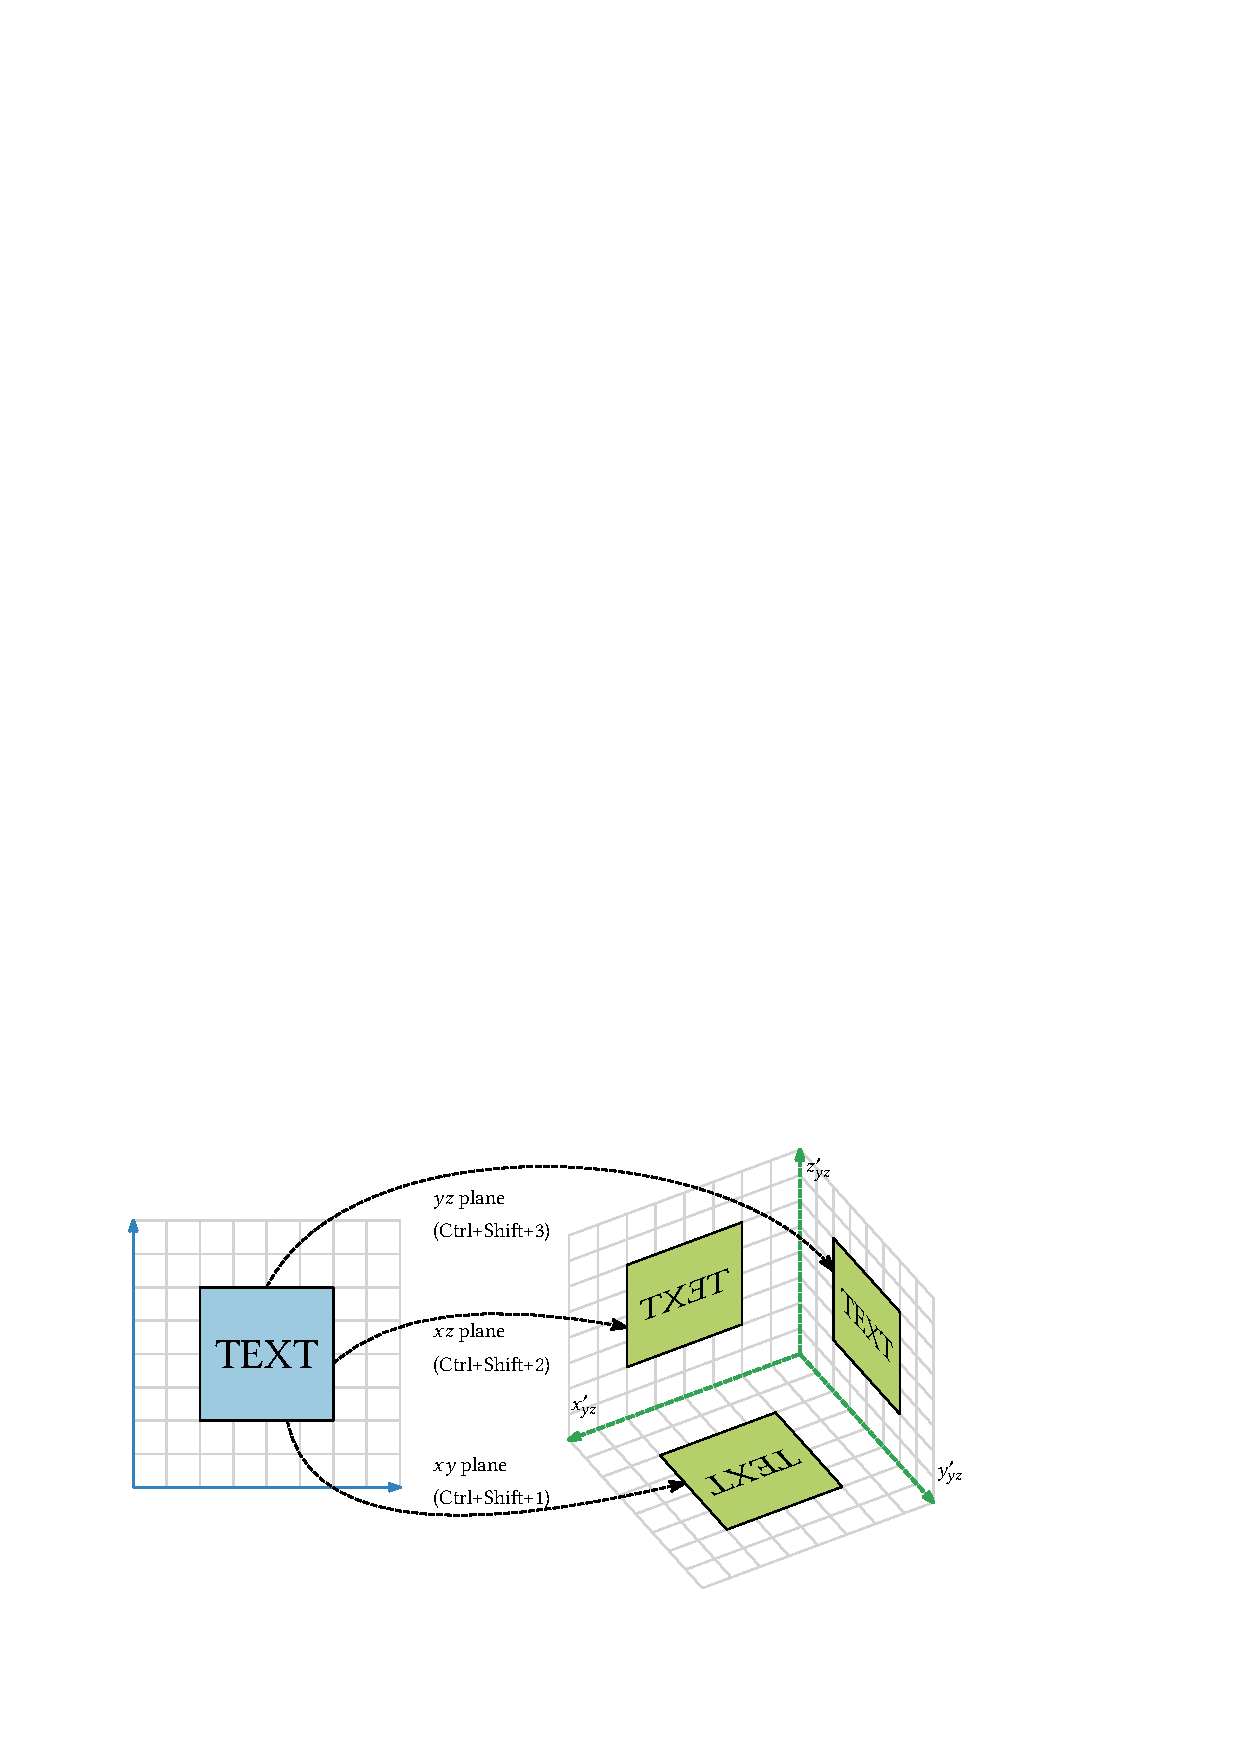
\includegraphics[scale=1]{pdf/projection_explained_default_v3.pdf}
\caption{Basic demonstration of the main three projection functions ($\phi=\SI{-60}{\degree}$, $\theta=\SI{40}{\degree}$, $\phi=\SI{0}{\degree}$).}
\label{fig:easy_explained}
\end{figure}

The projection without extra rotation is defined by three angles $ \phi $, $ \theta $ and $ \psi $ representing rotation of the coordinate system along the $ z $, $ y $ and $ x $ axis, respectively, see Fig.~\ref{fig:projection_explained_2}. Note that the effect of the last rotation is the same as performing a projection with $ \psi=\SI{0}{\degree} $ and then rotating the result in the drawing plane (i.e. using the Ctrl+R shortcut by the Goodies ipelet). The projection and math involved is described more deeply in the section below.

Angles $ \phi $, $ \theta $ and $ \psi $ can be set using a settings dialog. Values typed here are stored so there is no need for typing angle values before every projection (as this was an issue in the original version of this ipelet). However, whenever the ipe is closed, the values are lost. The dialog is also able to fill the values for a common special case of the axonometric projection -- isometric projection.

As mentioned above, the ipelet is able to perform a projection in all possible planes. These are described as planes rotated/tilted to $ xy $, $ yz $ or $ xz $ planes, the "extra rotations" along $ x $, $ y $ and $ z $ axii are described using angles $ \alpha $, $ \beta $ and $ \gamma $ respectively. These parameters are set in another settings dialog, the order from top to bottom determines the order of rotations and matters as matrix multiplication is not commutative (see the section below).

Performing an inverse operation is possible using the "Inverse operation" option. If the only transformation operation done to an object was using this ipelet, you can also revert the projection simply by removing matrix parameter if you edit the object as XML (right click, Edit as XML).

A useful feature might be using the projection on a (math) text, this is possible simply if the text is set as transformable.

\begin{figure}
\begin{center}
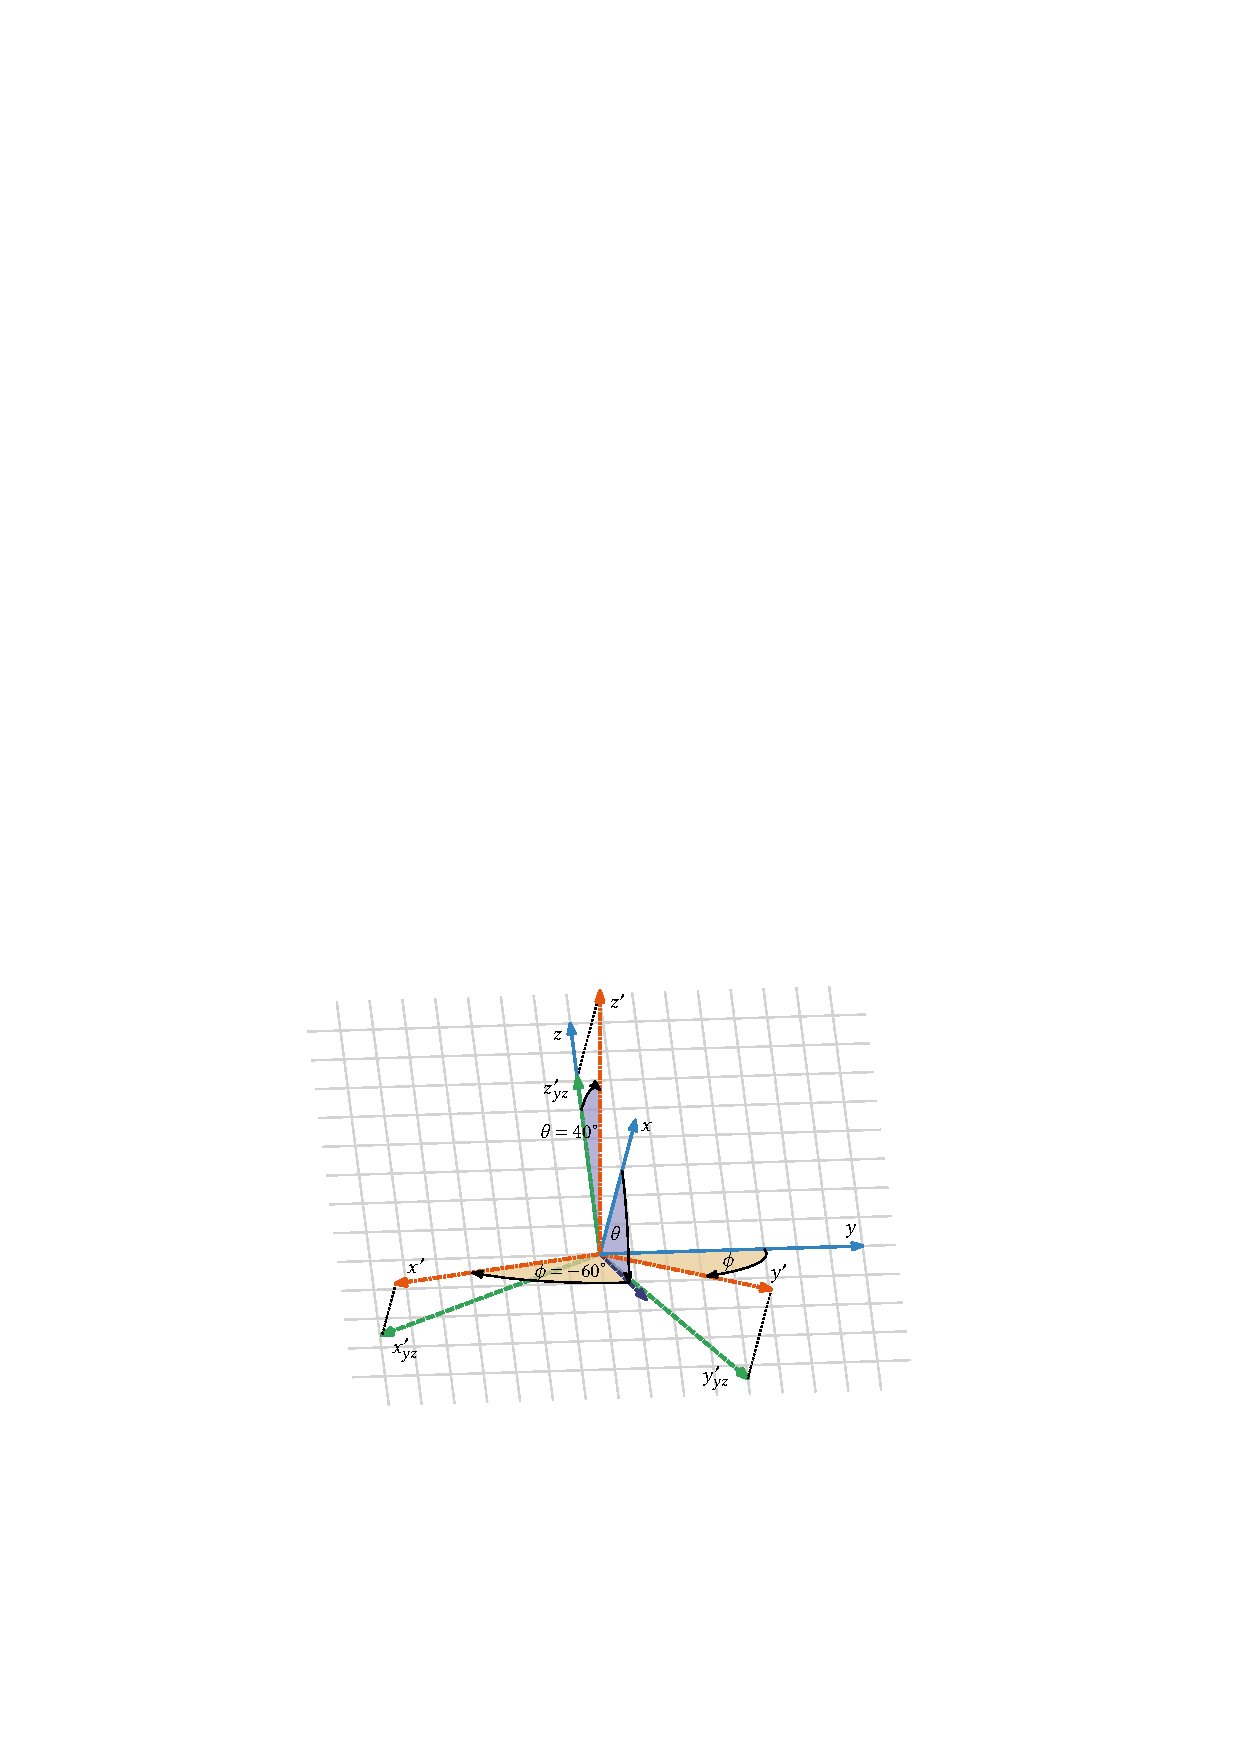
\includegraphics[scale=1]{pdf/projection_explained_2_v2.pdf}
\caption{Relation between the coordinate system of the drawing plane (blue) and the coordinate system in which the projected 3D geometry exists (red).}
\label{fig:projection_explained_2}
\end{center}
\end{figure}

%\begin{figure}
%\begin{center}
%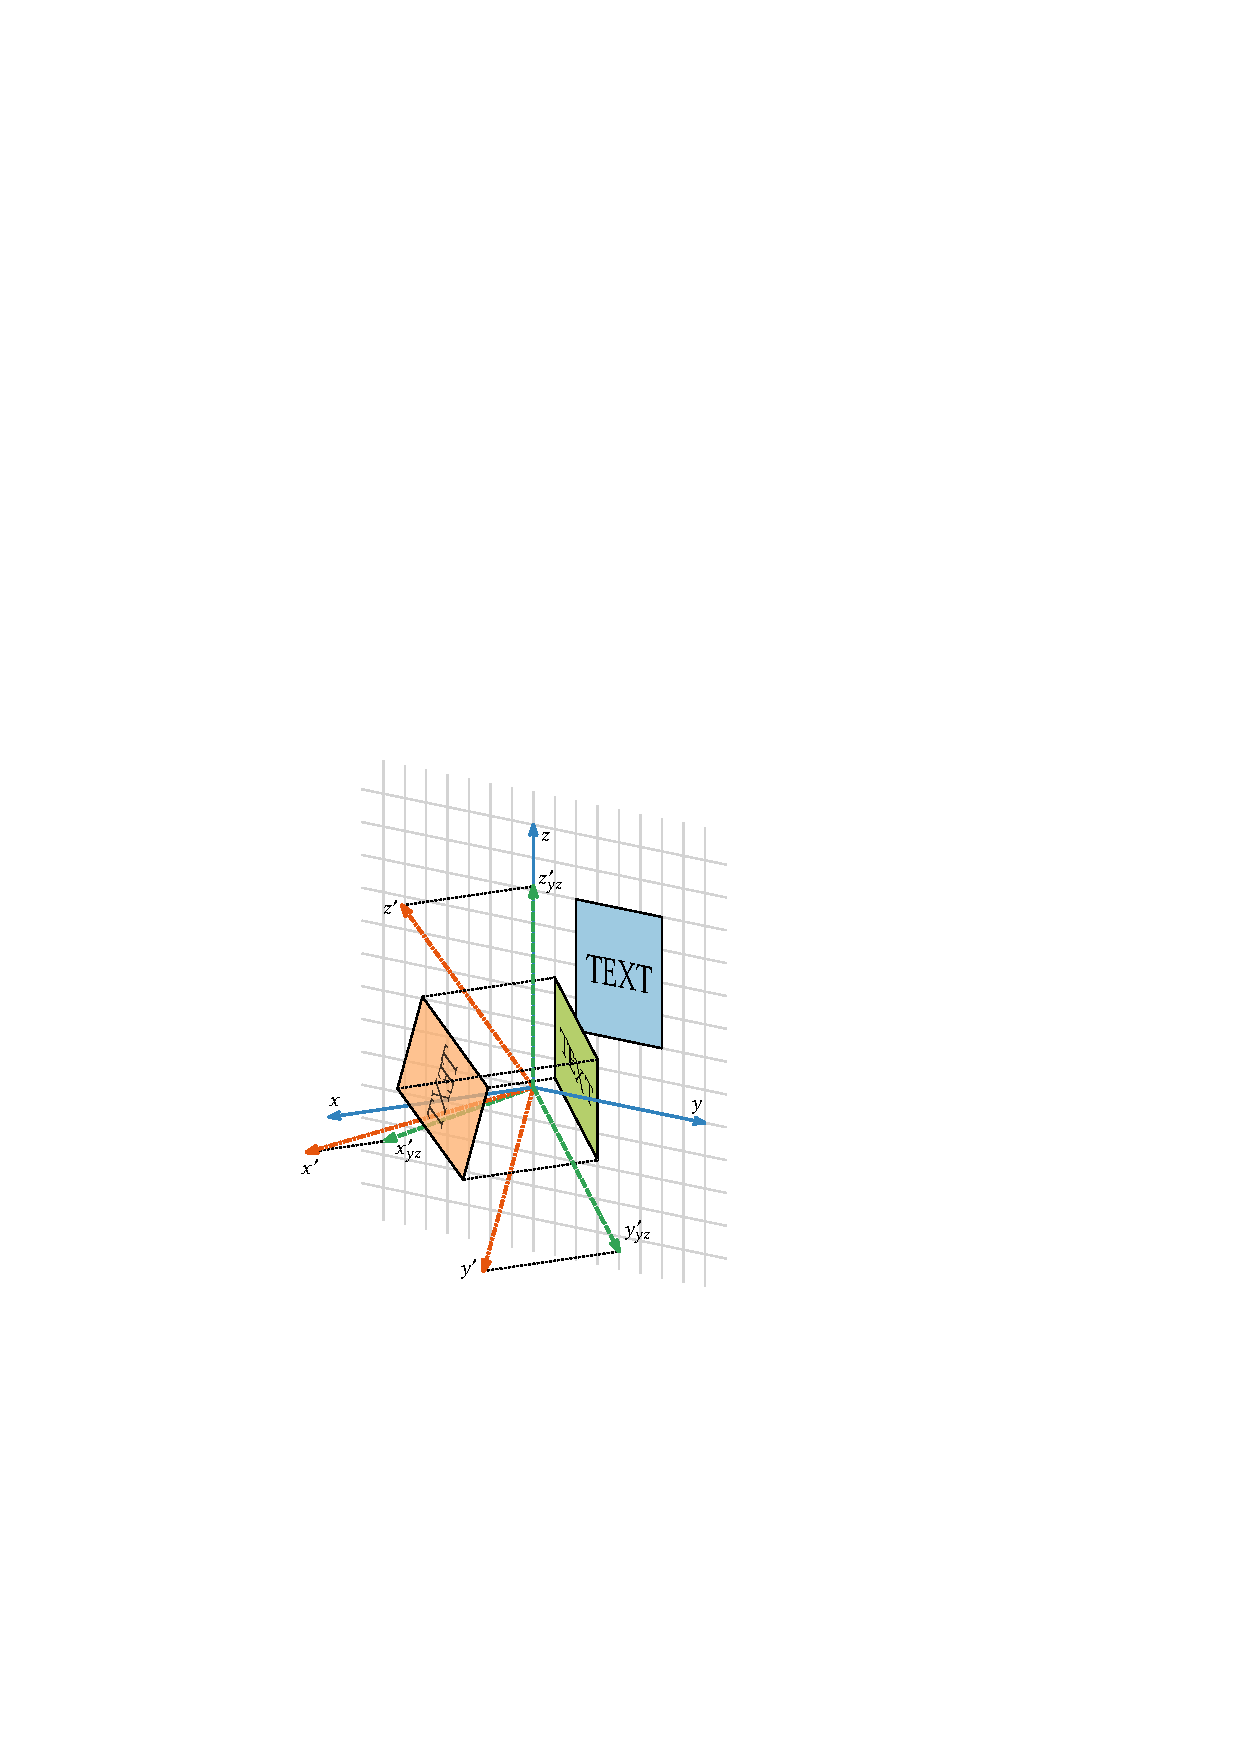
\includegraphics[scale=1]{pdf/projection_explained_1_v2.pdf}
%\caption{The original coordinate system (blue) is first rotated in the 3D space (red) and this new system is then projected onto the $yz$ plane (i.e. drawing plane). The red coordinate system can be referred as "the coordinate system" in which we are actually drawing the 3D geometry.}
%\label{fig:projection_explained_1}
%\end{center}
%\end{figure}


%\begin{figure}
%\begin{center}
%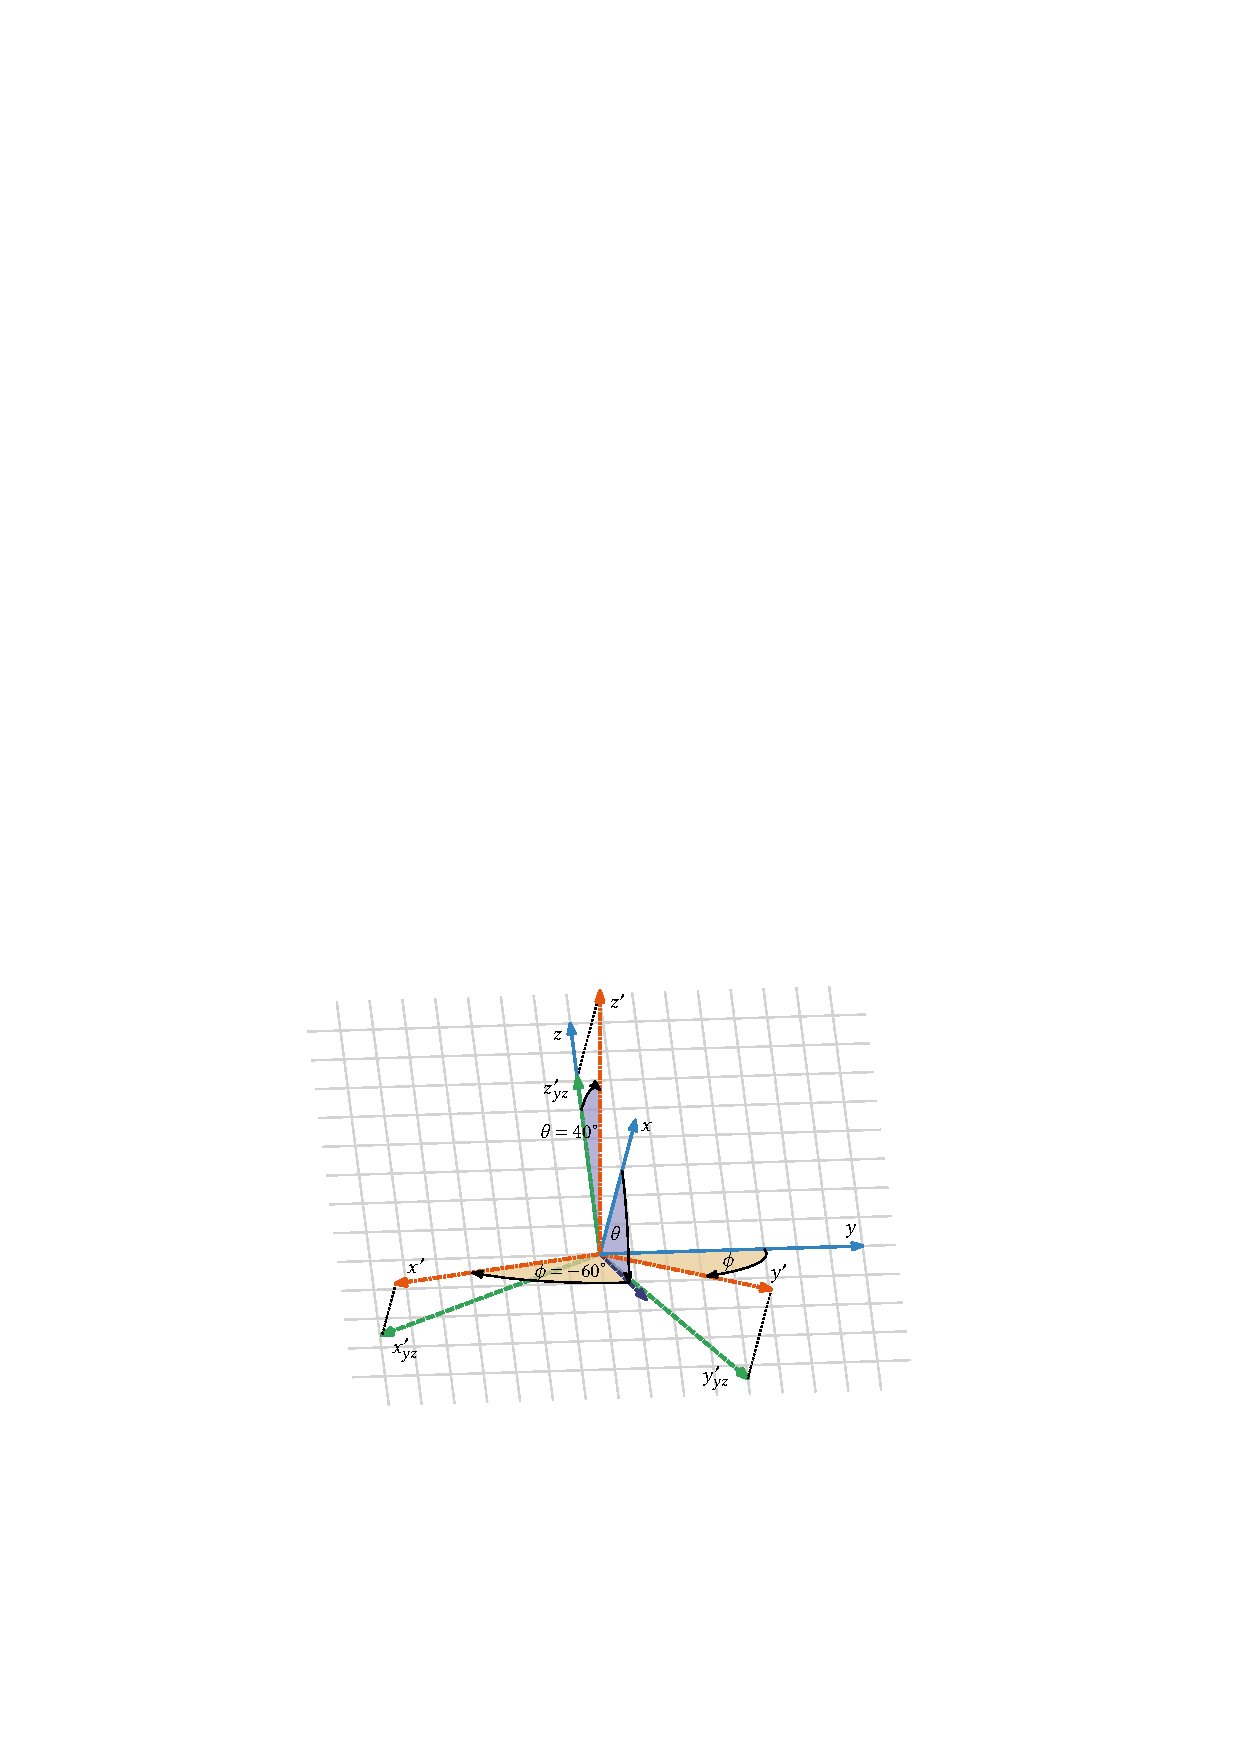
\includegraphics[scale=1]{pdf/projection_explained_2_v2.pdf}
%\caption{Projection explained -- definition of angles.}
%\label{fig:projection_explained_2}
%\end{center}
%\end{figure}

\section{A simple demo}

We will demonstrate usage of this ipelet on a simple cuboid with one vertex lying at the origin $(0,0,0)$. First, let's draw the bottom face lying in the $xy$ plane (Fig.~\ref{fig:demo1_a}). Next, we set the origin point (using F1 shortcut, Fig.~\ref{fig:demo1_b}), select the rectangle and do the projection onto the $ xy $ plane (Fig.~\ref{fig:demo1_c}) by either pressing Ctrl+Shift+1 or clicking "xy plane" in the menu. Similarly, the side and the back face is created, see Figs.~\ref{fig:demo1_d}--\ref{fig:demo1_g}. In the last step, the opposite faces are created using already projected faces by copying and translating these copies in the correct place using snapping on vertexes (Fig.~\ref{fig:demo1_h}).


% A simple demo: cuboid
\begin{figure}
\centering

\begin{subfigure}[t]{0.4\textwidth}
\centering
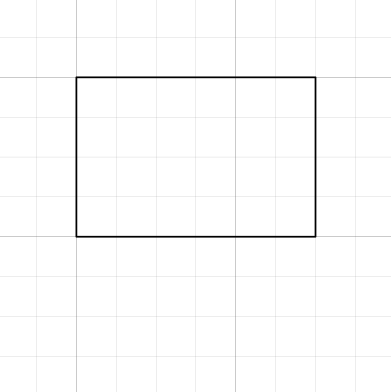
\includegraphics[scale=0.6]{png/demo_step1.png} 
\caption{Drawing the bottom face.}
\label{fig:demo1_a}
\end{subfigure}
\begin{subfigure}[t]{0.4\textwidth}
\centering
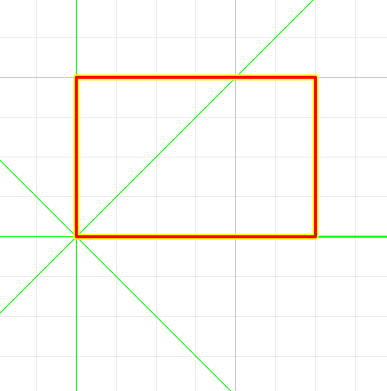
\includegraphics[scale=0.6]{png/demo_step2.png} 
\caption{Setting the origin (pressing F1) and selecting the rectangle.}
\label{fig:demo1_b}
\end{subfigure}

\begin{subfigure}[t]{0.4\textwidth}
\centering
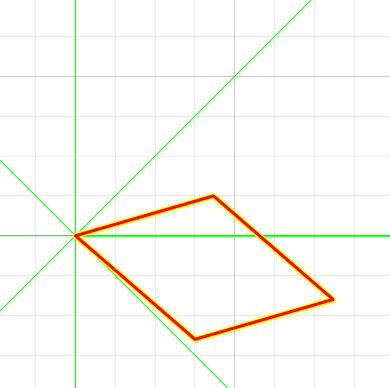
\includegraphics[scale=0.6]{png/demo_step3.png} 
\caption{Projection onto the $xy$ plane.}
\label{fig:demo1_c}
\end{subfigure}
\begin{subfigure}[t]{0.4\textwidth}
\centering
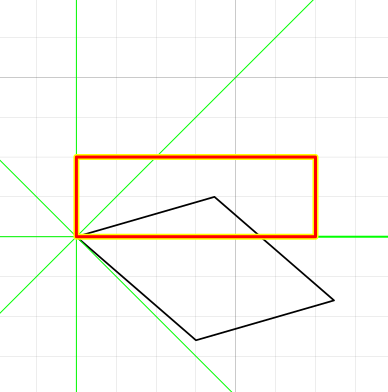
\includegraphics[scale=0.6]{png/demo_step4.png} 
\caption{Drawing the side face.}
\label{fig:demo1_d}
\end{subfigure}

\begin{subfigure}[t]{0.4\textwidth}
\centering
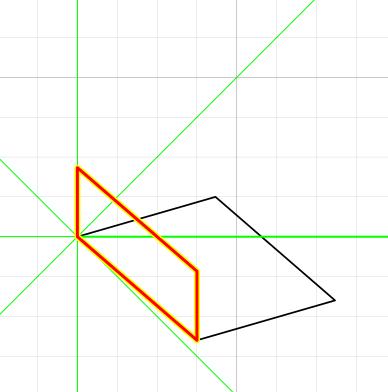
\includegraphics[scale=0.6]{png/demo_step5.png} 
\caption{Projection onto the $xz$ plane.}
\label{fig:demo1_e}
\end{subfigure}
\begin{subfigure}[t]{0.4\textwidth}
\centering
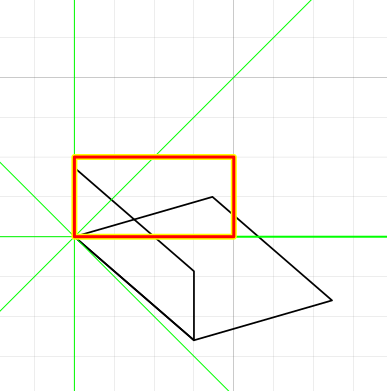
\includegraphics[scale=0.6]{png/demo_step6.png} 
\caption{Drawing the last face.}
\label{fig:demo1_f}
\end{subfigure}

\begin{subfigure}[t]{0.4\textwidth}
\centering
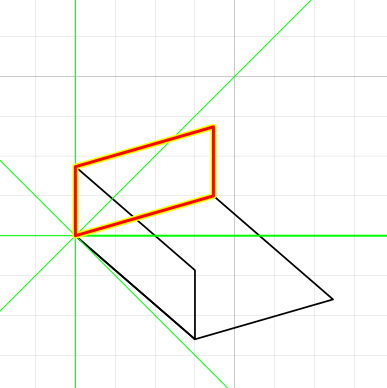
\includegraphics[scale=0.6]{png/demo_step7.png} 
\caption{Projection onto the $yz$ plane.}
\label{fig:demo1_g}
\end{subfigure}
\begin{subfigure}[t]{0.4\textwidth}
\centering
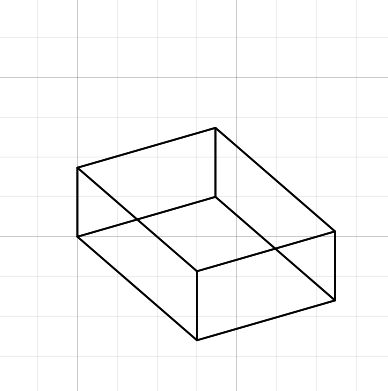
\includegraphics[scale=0.6]{png/demo_step8.png} 
\caption{Opposite faces are made using the copy and translate functions.}
\label{fig:demo1_h}
\end{subfigure}

\caption{A simple demo -- drawing a cuboid using the default axonometric projection with angles $ \phi=\SI{30}{\degree} $, $ \theta=\SI{30}{\degree} $, $ \psi=\SI{0}{\degree} $.}
\end{figure}


\section{Mathematical background}

%The original coordinate system (blue) is first rotated in the 3D space (red) and this new system is then projected onto the $yz$ plane (i.e. drawing plane). The red coordinate system can be referred as "the coordinate system" in which we are actually drawing the 3D geometry.

An axonometric projection is a linear projection $ \mathbb{R}^{3}\rightarrow\mathbb{R}^{2} $, we would like to describe this projection. The $ \mathbb{R}^{3} $ is described using orthonormal basis
\begin{equation}
\vec{\i}=
\begin{pmatrix}
1 \\
0 \\
0 \\
\end{pmatrix}, \quad
\vec{\j}=
\begin{pmatrix}
0 \\
1 \\
0 \\
\end{pmatrix}, \quad
\vec{k}=
\begin{pmatrix}
0 \\
0 \\
1 \\
\end{pmatrix}.
\end{equation}
Let's choose the $ yz $ plane as the $ \mathbb{R}^{2} $ (we would like to have the $ z $ axis pointing upwards and the $ x $ axis pointing out of the drawing plane). Now the projection of an object projected in defined $ \mathbb{R}^{2} $ would be simply the projection in the $ yz $ plane, i.e.
\begin{equation}
\begin{pmatrix}
y' \\
z' \\
\end{pmatrix}
=
\begin{pmatrix}
0 & 1 & 0 \\
0 & 0 & 1 \\
\end{pmatrix}
\cdot
\begin{pmatrix}
x \\
y \\
z \\
\end{pmatrix}
=
\begin{pmatrix}
y \\
z \\
\end{pmatrix}.
\end{equation}
If we would like to create an actual axonometric projection (and not that simple degenerate case), we have to "look at the coordinate system with the object from a different direction". This can be simply achieved by rotating the coordinate system including the object before the $ \mathbb{R}^{3}\rightarrow\mathbb{R}^{2} $ projection, which can be done using rotation matrices
\begin{equation}
R_{x}(\omega)=
\begin{pmatrix}
1 & 0 & 0 \\
0 & \cos(\omega) & -\sin(\omega) \\
0 & \sin(\omega) & \cos(\omega) \\
\end{pmatrix},
\end{equation}
\begin{equation}
R_{y}(\omega)=
\begin{pmatrix}
\cos(\omega) & 0 & \sin(\omega) \\
0 & 1 & 0 \\
-\sin(\omega) & 0 & \cos(\omega) \\
\end{pmatrix},
\end{equation}
\begin{equation}
R_{z}(\omega)=
\begin{pmatrix}
\cos(\omega) & -\sin(\omega) & 0 \\
\sin(\omega) & \cos(\omega) & 0 \\
0 & 0 & 1 \\
\end{pmatrix},
\end{equation}
which rotate along $ x $, $ y $ and $ z $ axis, respectively. In order to keep the direction of the $ z $ axis, we will rotate first along the $ z $ axis by angle $ \phi $ and than along the $ y $ axis by angle $ \theta $, see Fig.~\ref{fig:projection_explained_2} and Fig.~\ref{fig:projection_explained_1}. If we don't mind keeping the direction of the $ z $ axis, we can additionally rotate along the $ x $ axis by angle $ \psi $.


% Some scratch texts before the rotation matrices:

%By $ \mathbb{R}^{3} $ we mean a "standard" 3D space with orthogonal axes $ x,y,z $. $ \mathbb{R}^{2} $ will be our drawing plane and we will define it on the $ yz $ plane.

%Generally speaking, we would like to make a projection of an object on any plane in space, however, as all parallel planes will give us the same result, we can consider only all planes passing through the origin. We can think about these planes as $ yz $ planes of different coordinate systems. Obviously, we can 

%of $ xy $, $ xz $ and $ yz $ plane in which we can usually easily draw an object. As we defined the system so far, the projection of an object onto the $ yz $ plane would be simply just the projection of the $ yz $ plane. In order to make a projection of the coordinate system from any direction, we will rotate the whole coordinate system using rotation matrices

\begin{figure}
\begin{center}
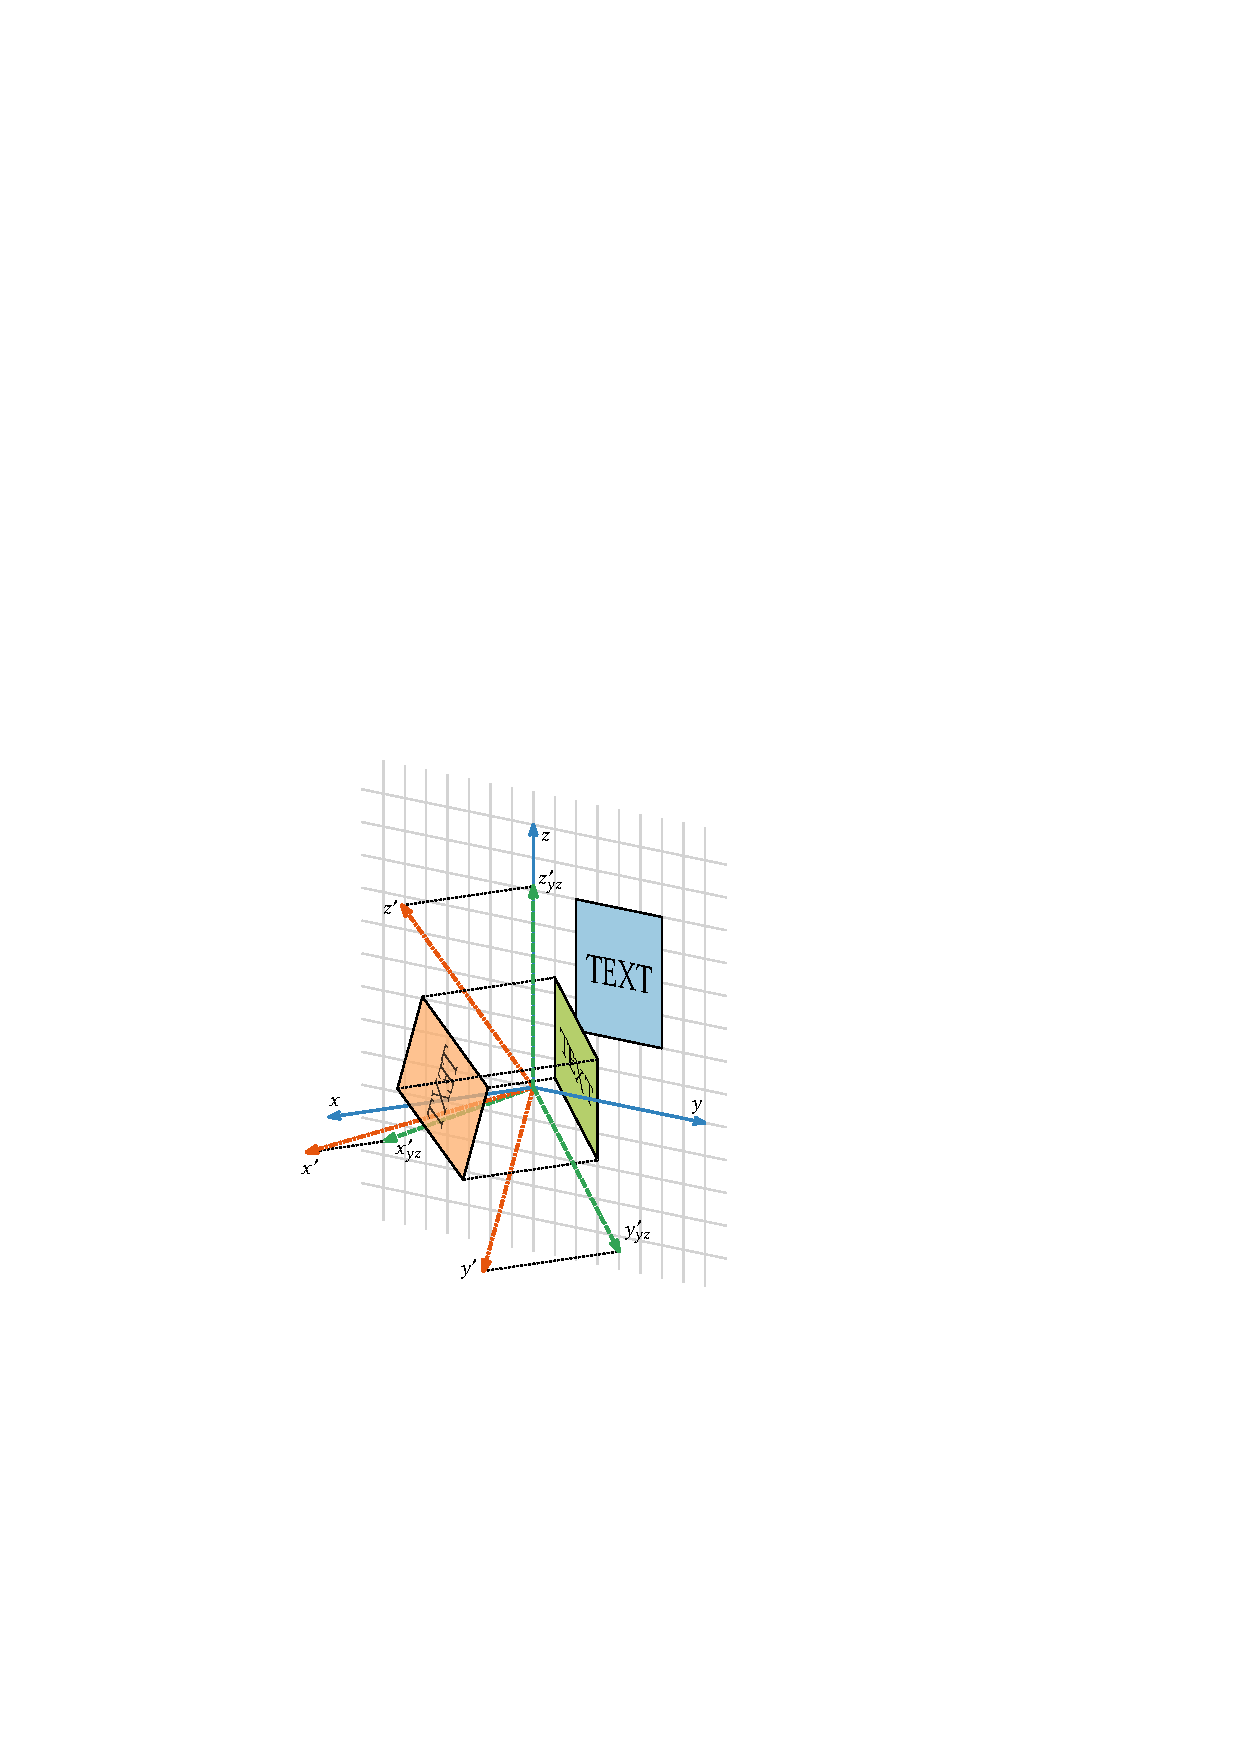
\includegraphics[scale=1]{pdf/projection_explained_1_v2.pdf}
\caption{The original coordinate system (blue) is first rotated in the 3D space (red) and this new system is then projected onto the $yz$ plane -- drawing plane (green). In this case, $yz$ plane projection is demonstrated.}
\label{fig:projection_explained_1}
\end{center}
\end{figure}

If we would like to to make a projection of planes tilted to $ xy $, $ xz $ or $ yz $ plane, we can do so by rotating the coordinate system before performing rotations described in the previous paragraph. We define angles $ \alpha $, $ \beta $ and $ \gamma $ describing rotation along the $ x $, $ y $ and $ z $ axes respectively. When doing extra rotations, user can define three matrices
\begin{equation}
R_{1}=
\begin{cases}
R_x(\alpha) \\
R_y(\beta) \\
R_z(\gamma)
\end{cases}, \quad
R_{2}=
\begin{cases}
R_x(\alpha) \\
R_y(\beta) \\
R_z(\gamma)
\end{cases}, \quad
R_{3}=
\begin{cases}
R_x(\alpha) \\
R_y(\beta) \\
R_z(\gamma)
\end{cases}.
\end{equation}
Then, we can define a matrix describing the whole transformation using all the rotations mentioned
\begin{equation}
M=
\begin{cases}
R_x(\psi) \cdot R_y(\theta) \cdot R_z(\phi) & \text{for default projection} \\
R_x(\psi) \cdot R_y(\theta) \cdot R_z(\phi) \cdot R_3 \cdot R_2 \cdot R_1 & \text{for additional rotation} \\
\end{cases}.
\end{equation}

The transformation using the matrix $ M $ on any given point can be written as
\begin{equation}
\begin{pmatrix}
x' \\
y' \\
z' \\
\end{pmatrix}
= M\cdot
\begin{pmatrix}
x \\
y \\
z \\
\end{pmatrix}.
\end{equation}
Let's label the matrix elements
\begin{equation}
M=
\begin{pmatrix}
m_{11} & m_{12} & m_{13} \\
m_{21} & m_{22} & m_{23} \\
m_{31} & m_{32} & m_{33} \\
\end{pmatrix}
=
\begin{pmatrix}
\vec{\i}_{M} & \vec{\j}_{M} & \vec{k}_{M}
\end{pmatrix},
\end{equation}
$\vec{\i}_{M}$, $\vec{\j}_{M}$ and $\vec{k}_{M}$ are basis vectors of the transformed coordinate system (they are transformed basis vectors in different words). The $ \mathbb{R}^{3}\rightarrow\mathbb{R}^{2} $ linear projection onto the $ yz $ plane can be thus written as
\begin{equation}
\begin{pmatrix}
0 \\
y' \\
z' \\
\end{pmatrix}
=
\begin{pmatrix}
0 & 0 & 0 \\
m_{21} & m_{22} & m_{23} \\
m_{31} & m_{32} & m_{33} \\
\end{pmatrix}
\cdot
\begin{pmatrix}
x \\
y \\
z \\
\end{pmatrix},
\end{equation}
or simply
\begin{equation}
\begin{pmatrix}
y' \\
z' \\
\end{pmatrix}
=
\begin{pmatrix}
m_{21} & m_{22} & m_{23} \\
m_{31} & m_{32} & m_{33} \\
\end{pmatrix}
\cdot
\begin{pmatrix}
x \\
y \\
z \\
\end{pmatrix},
\end{equation}
we will label vectors in the matrix as
\begin{equation}
\begin{pmatrix}
m_{21} \\
m_{31} \\
\end{pmatrix}
=\vec{\i}_{M,yz}, \quad
\begin{pmatrix}
m_{22} \\
m_{32} \\
\end{pmatrix}
=\vec{\j}_{M,yz}, \quad
\begin{pmatrix}
m_{23} \\
m_{33} \\
\end{pmatrix}
=\vec{k}_{M,yz},
\end{equation}
$\vec{\i}_{M,yz}$, $\vec{\j}_{M,yz}$ and $\vec{k}_{M,yz}$ are projections of the transformed basis vectors. Using these vectors, the actual $ \mathbb{R}^{2}\rightarrow\mathbb{R}^{2} $ transformation in Ipe can be done. Ipe uses for transformations matrix defined as
\begin{equation}
M_{\text{Ipe}} =
\begin{pmatrix}
a & c & s \\
b & d & t \\
\end{pmatrix},
\end{equation}
so coordinate values of an object are transformed as
\begin{equation}
\begin{pmatrix}
x' \\
y' \\
\end{pmatrix}
=
\begin{pmatrix}
a & c & s \\
b & d & t \\
\end{pmatrix}
\cdot
\begin{pmatrix}
x \\
y \\
1 \\
\end{pmatrix}
=
\begin{pmatrix}
ax+cy+s \\
bx+dy+t \\
\end{pmatrix}
\end{equation}
(now $x,y,x',y'$ refers to the 2D coordinates of the Ipe drawing plane).

The ipe transformation matrix is then finally obtained as
\begin{equation}
M_{\text{Ipe,axonometric}} =
\begin{cases}
\begin{pmatrix}
\vec{\i}_{M,yz} & \vec{\j}_{M,yz} & \vec{0}
\end{pmatrix}
=
\begin{pmatrix}
m_{21} & m_{22} & 0 \\
m_{31} & m_{32} & 0 \\
\end{pmatrix}
& \text{for $xy$ plane,} \\
\begin{pmatrix}
\vec{\i}_{M,yz} & \vec{k}_{M,yz} & \vec{0}
\end{pmatrix}
=
\begin{pmatrix}
m_{21} & m_{23} & 0 \\
m_{31} & m_{33} & 0 \\
\end{pmatrix}
& \text{for $xz$ plane,} \\
\begin{pmatrix}
\vec{\j}_{M,yz} & \vec{k}_{M,yz} & \vec{0}
\end{pmatrix}
=
\begin{pmatrix}
m_{22} & m_{23} & 0 \\
m_{32} & m_{33} & 0 \\
\end{pmatrix}
& \text{for $yz$ plane.} \\
\end{cases}
\end{equation}

%\section*{Appendix A: Dialog windows}
%\addcontentsline{toc}{section}{Appendix A: Dialog windows}
%
%\begin{figure}[h]
%\begin{center}
%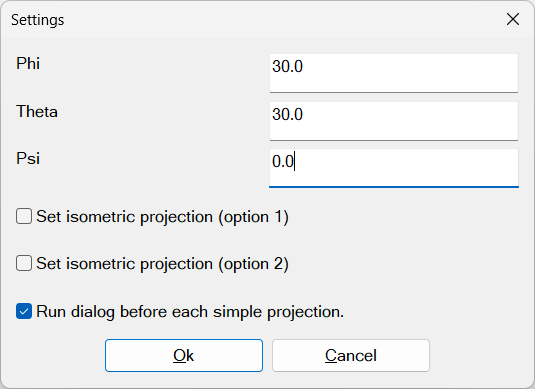
\includegraphics[scale=0.5]{png/gui/settings_main.png}
%\caption{Main settings dialog.}
%\label{fig:settings_gui_noextra}
%\end{center}
%\end{figure}
%
%\begin{figure}[h]
%\begin{center}
%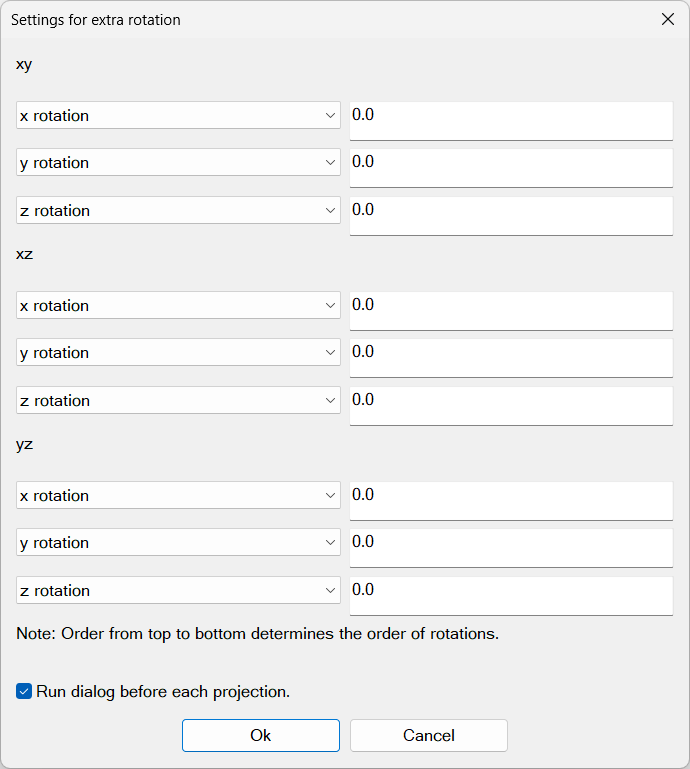
\includegraphics[scale=0.5]{png/gui/settings_extra_rot.png}
%\caption{Settings dialog (full) for additional rotation / extra tilt angles.}
%\label{fig:settings_gui_withextra}
%\end{center}
%\end{figure}
%
%\begin{figure}[h]
%\begin{center}
%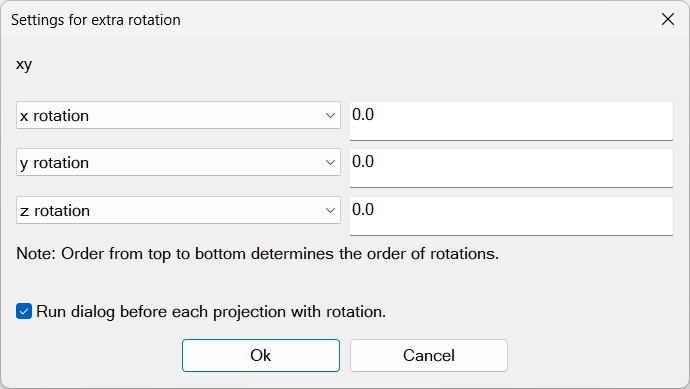
\includegraphics[scale=0.55]{png/gui/settings_extra_rot_lite.png}
%\caption{Settings dialog or extra rotation ("lite" version).}
%\label{fig:settings_gui_withextra_lite}
%\end{center}
%\end{figure}

\clearpage
\section*{Appendix A: Extra rotations}
\label{sec:appendix_A}
\addcontentsline{toc}{section}{Appendix A: Extra rotations}

The effect of extra rotation is demonstrated below for extra rotation around one axis at a time.

%\begin{figure}[h]
\begin{center}
%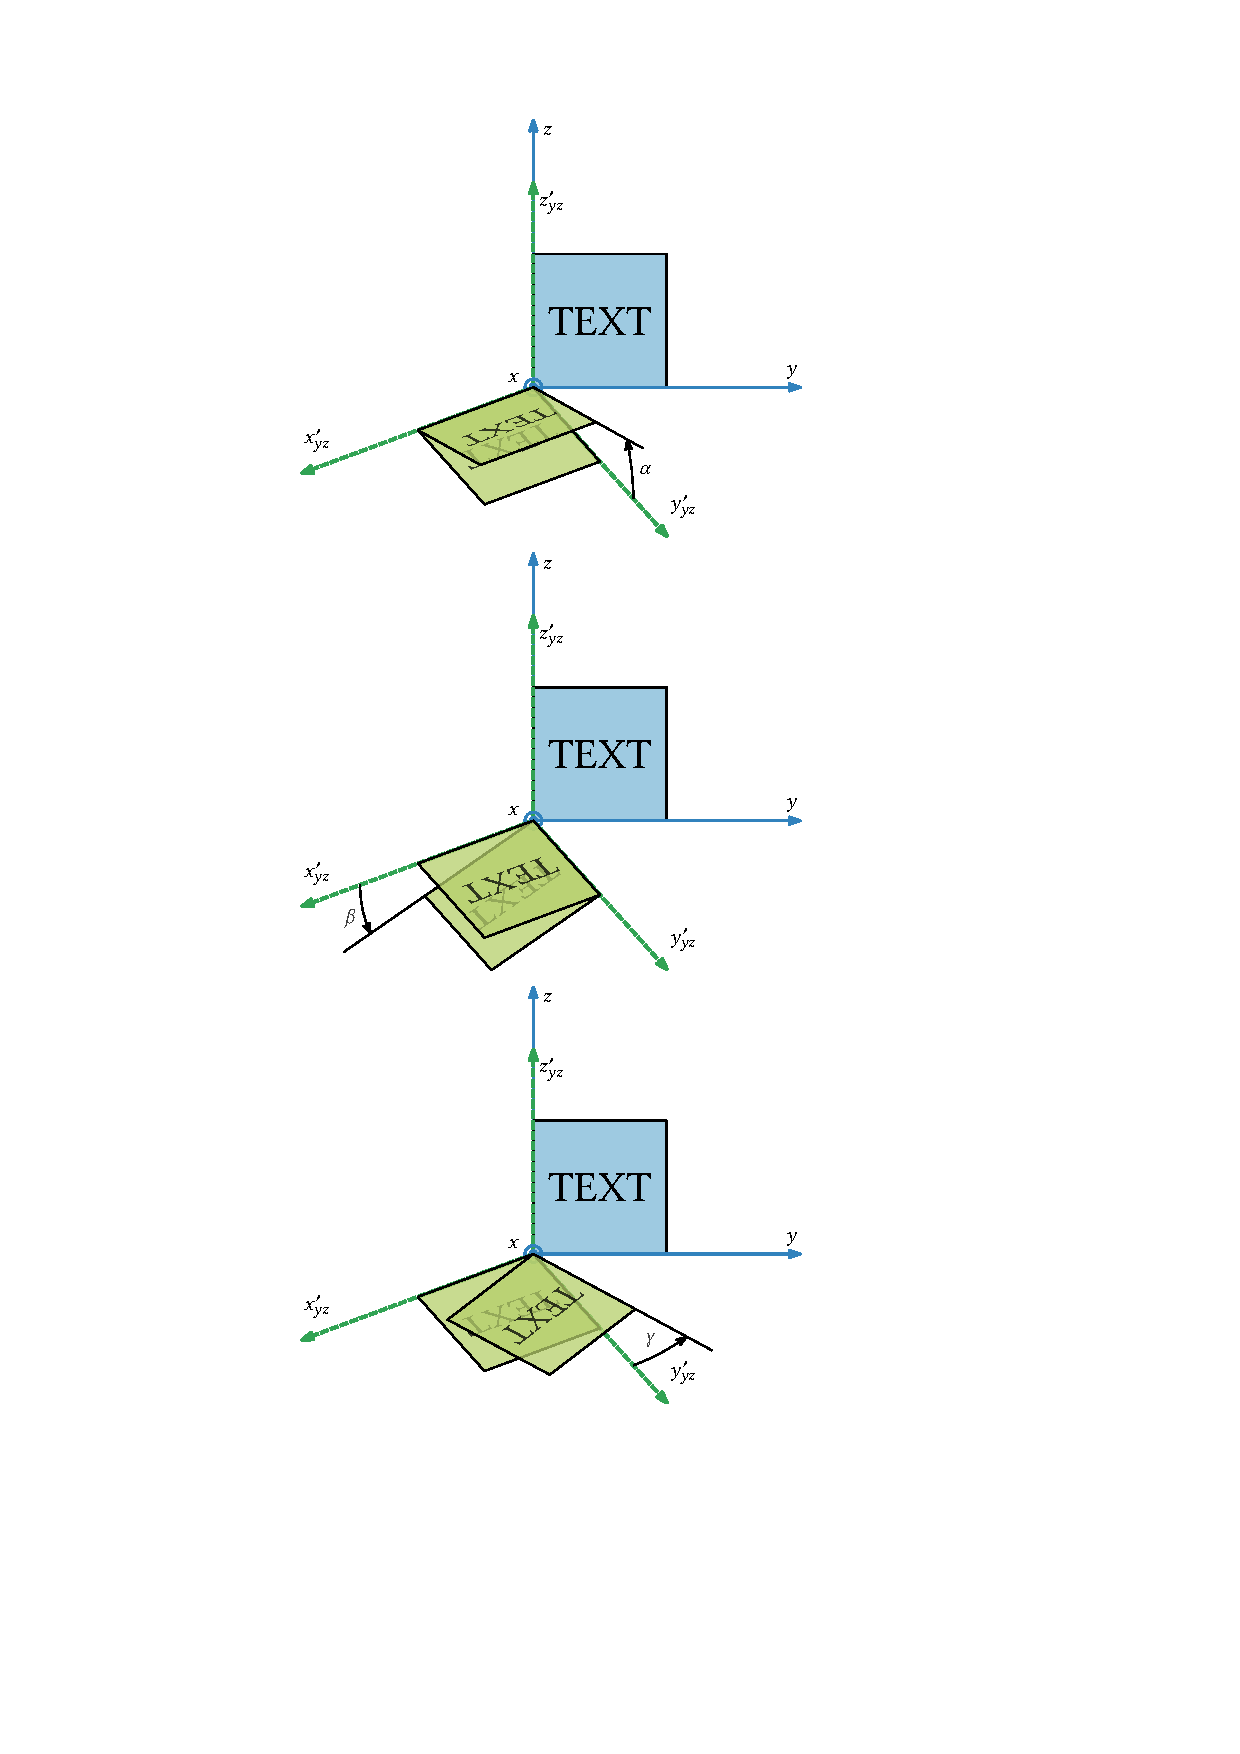
\includegraphics[scale=0.6]{pdf/projection_explained_extra_rot_xy_v2.pdf}
%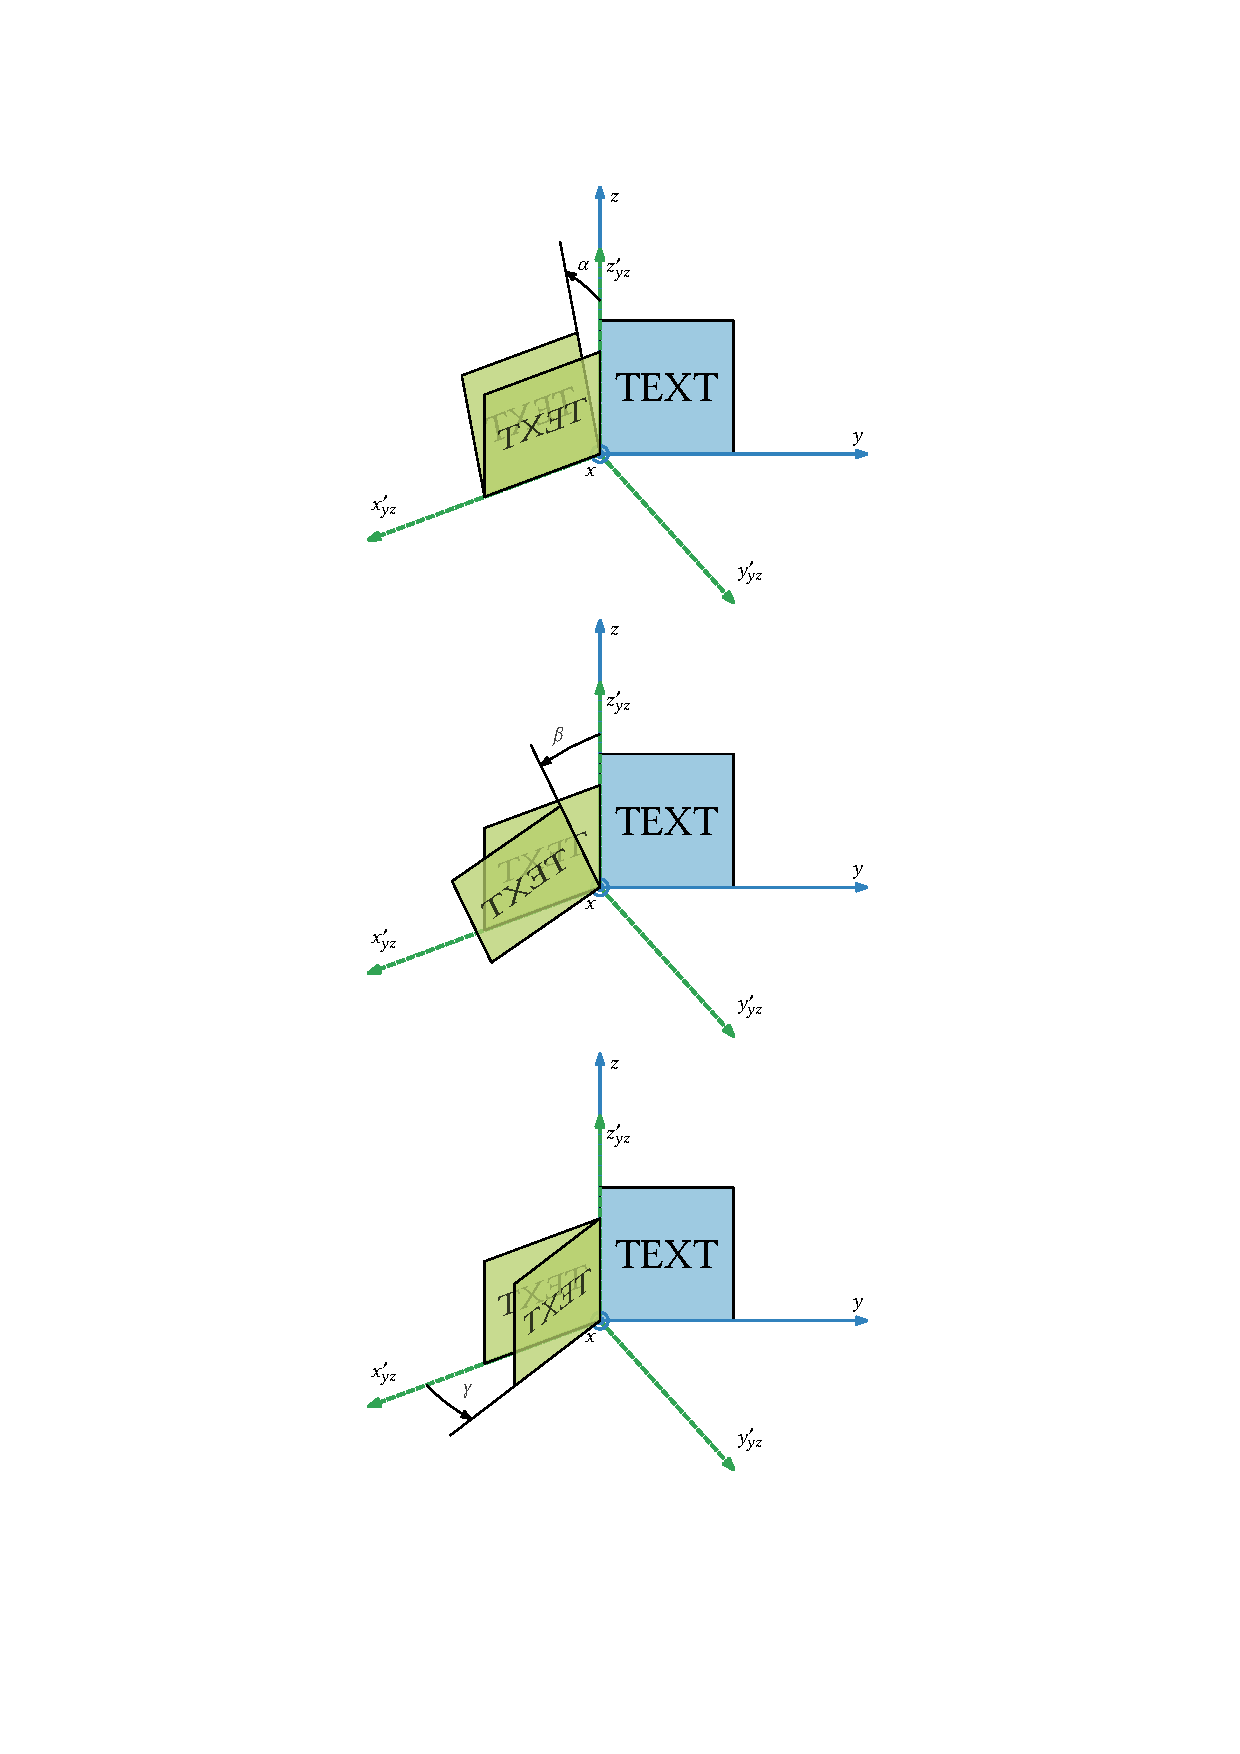
\includegraphics[scale=0.6]{pdf/projection_explained_extra_rot_xz_v2.pdf}
%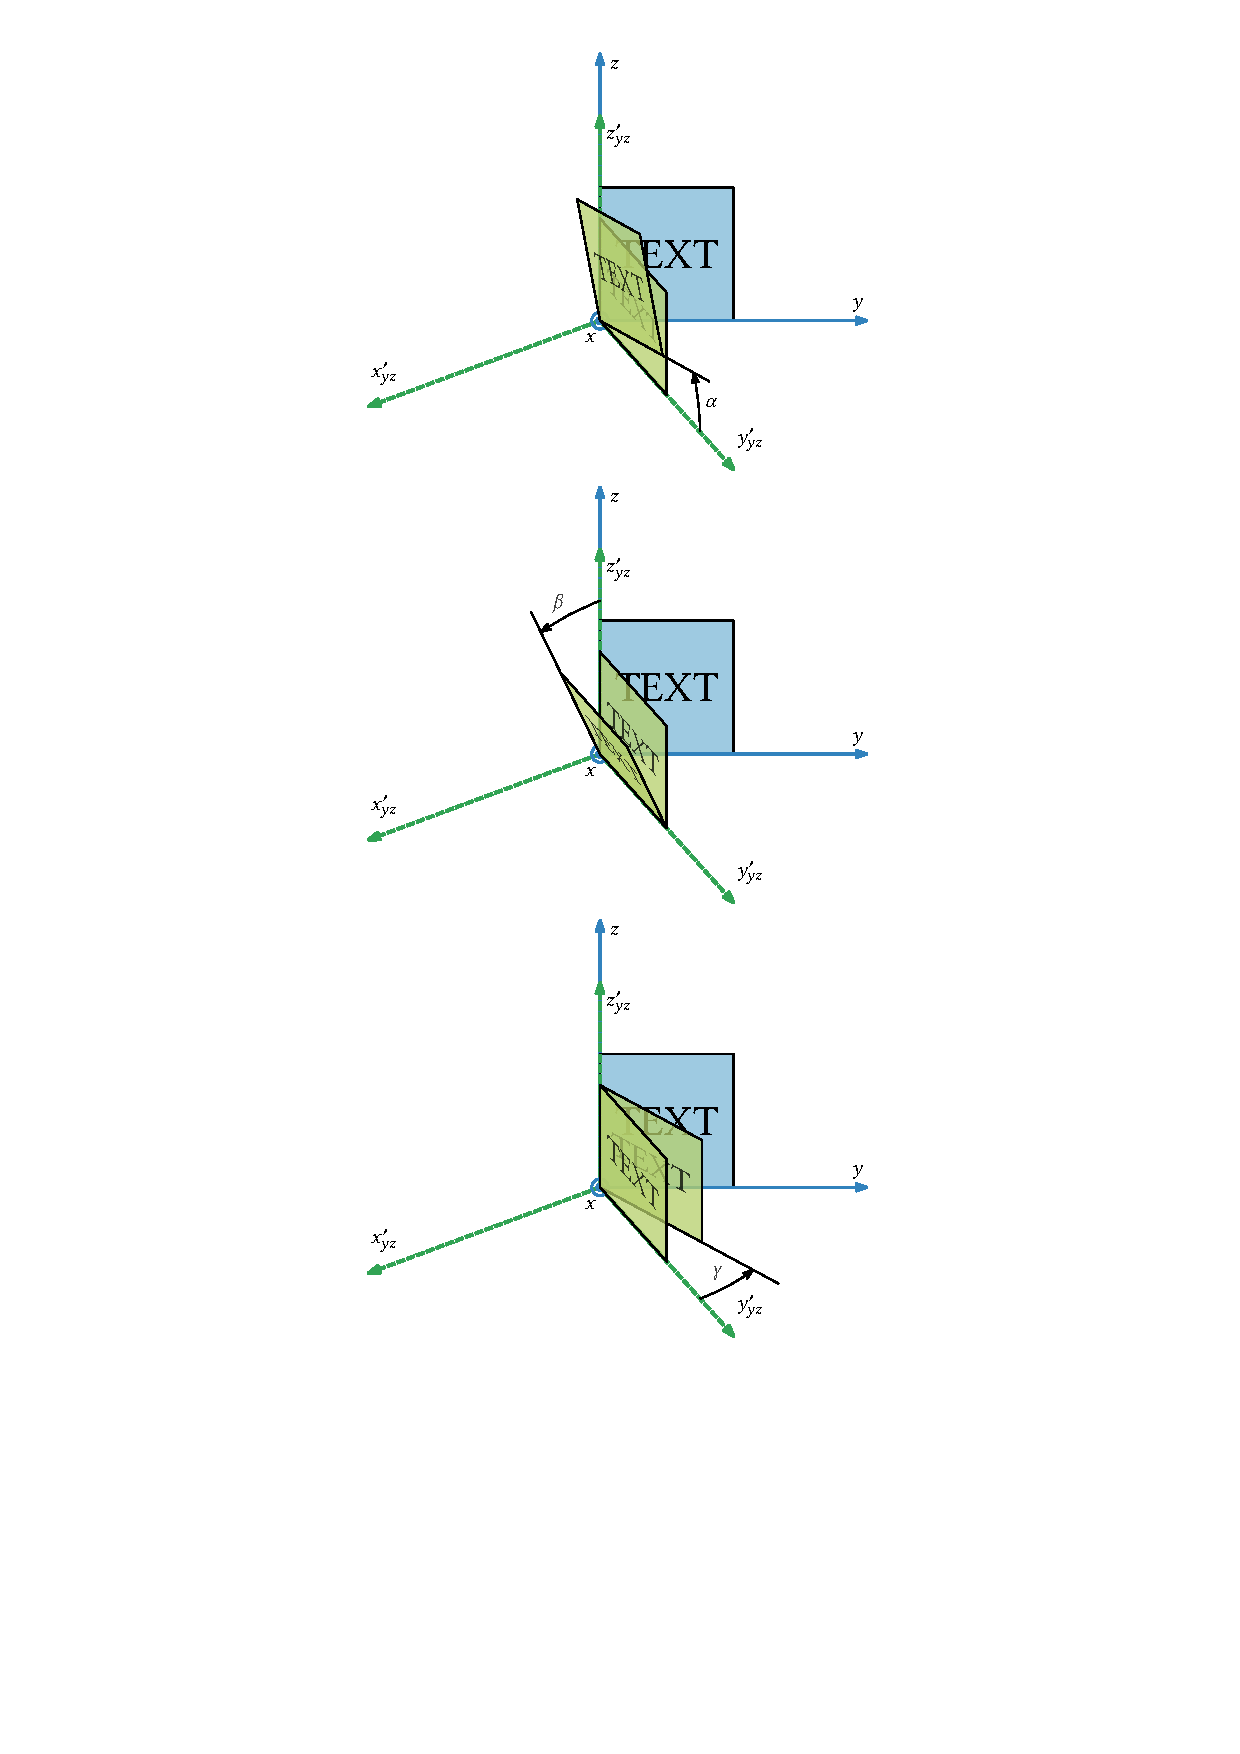
\includegraphics[scale=0.6]{pdf/projection_explained_extra_rot_yz_v2.pdf}

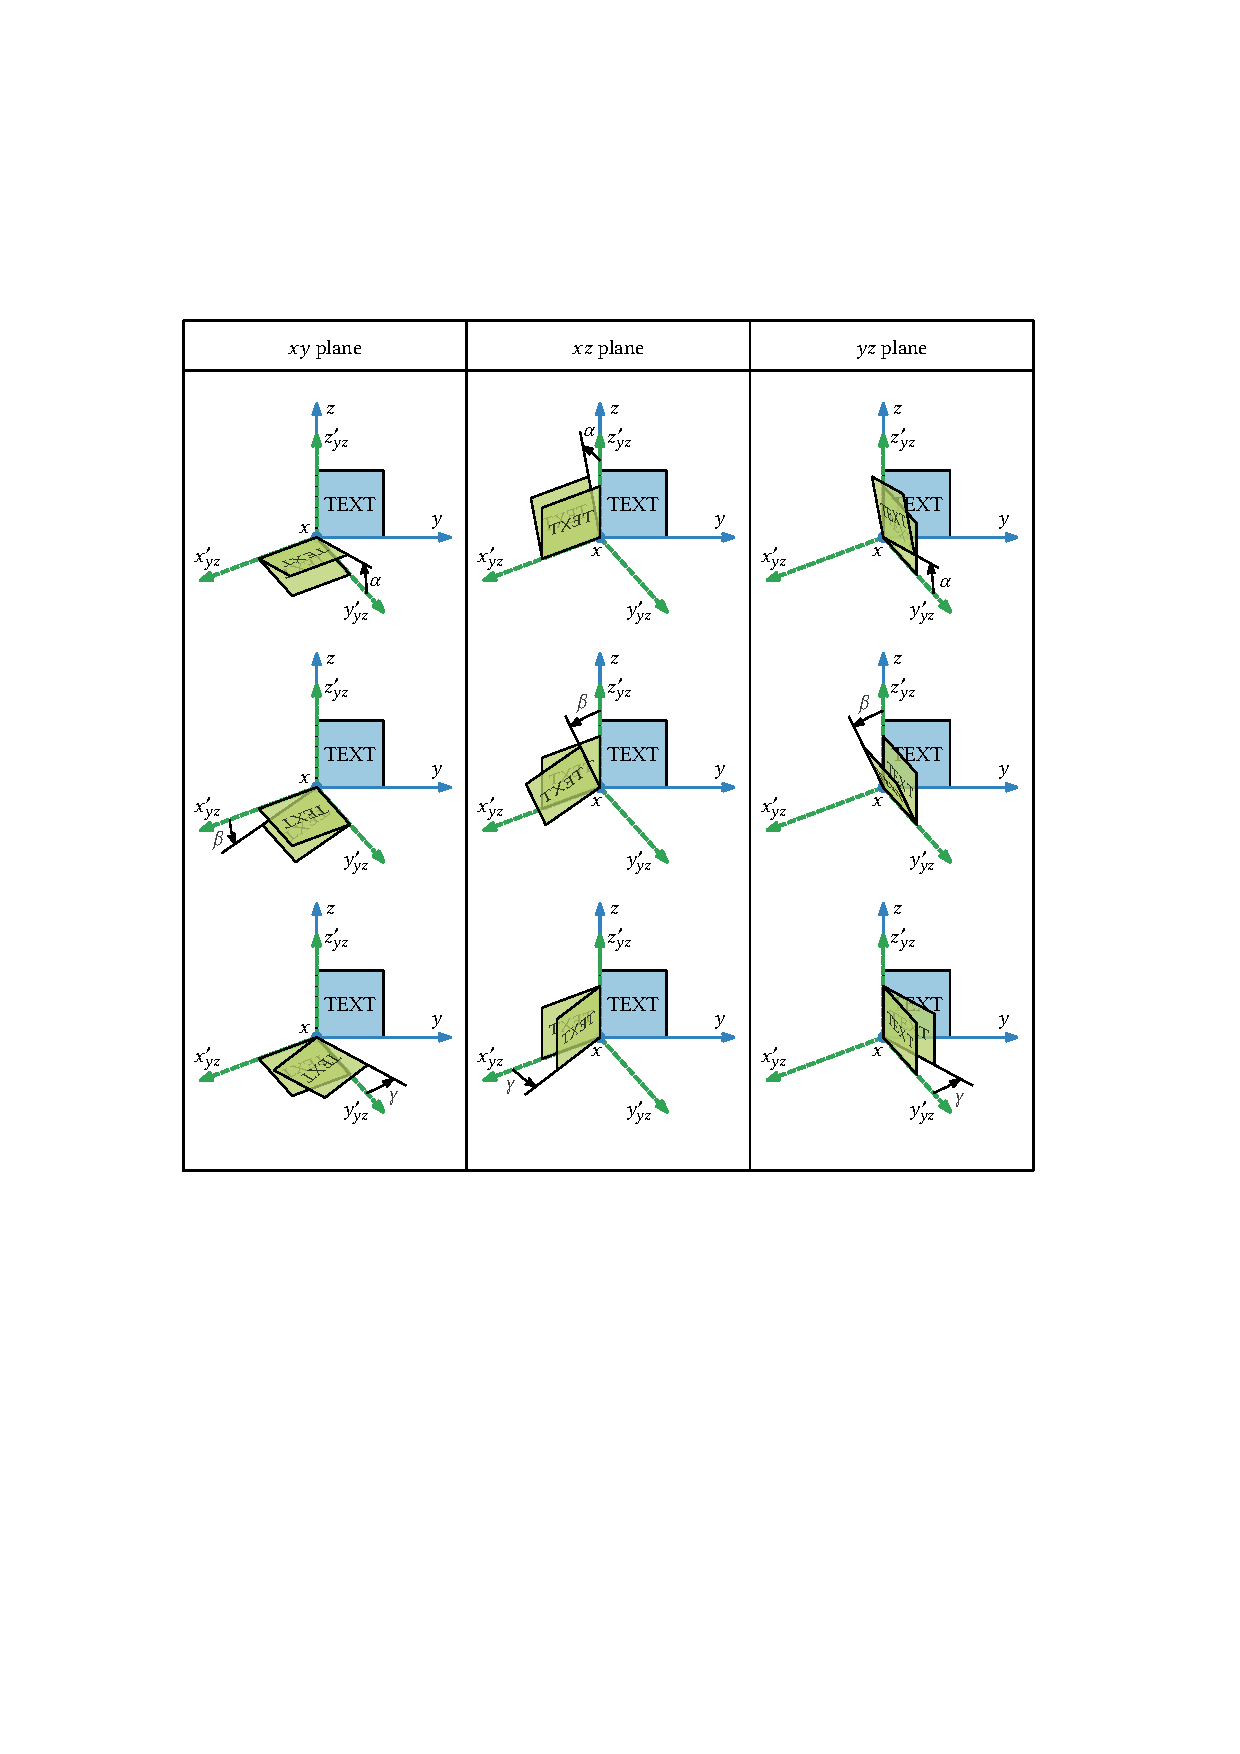
\includegraphics[scale=1.0]{pdf/projection_explained_extra_rot_matrix.pdf}
%\caption{Extra rotation for projection onto the $xy$, $xz$ and $yz$ plane.}
%\label{fig:extra_rot_matrix}
\end{center}
%\end{figure}

%\begin{figure}
%\begin{center}
%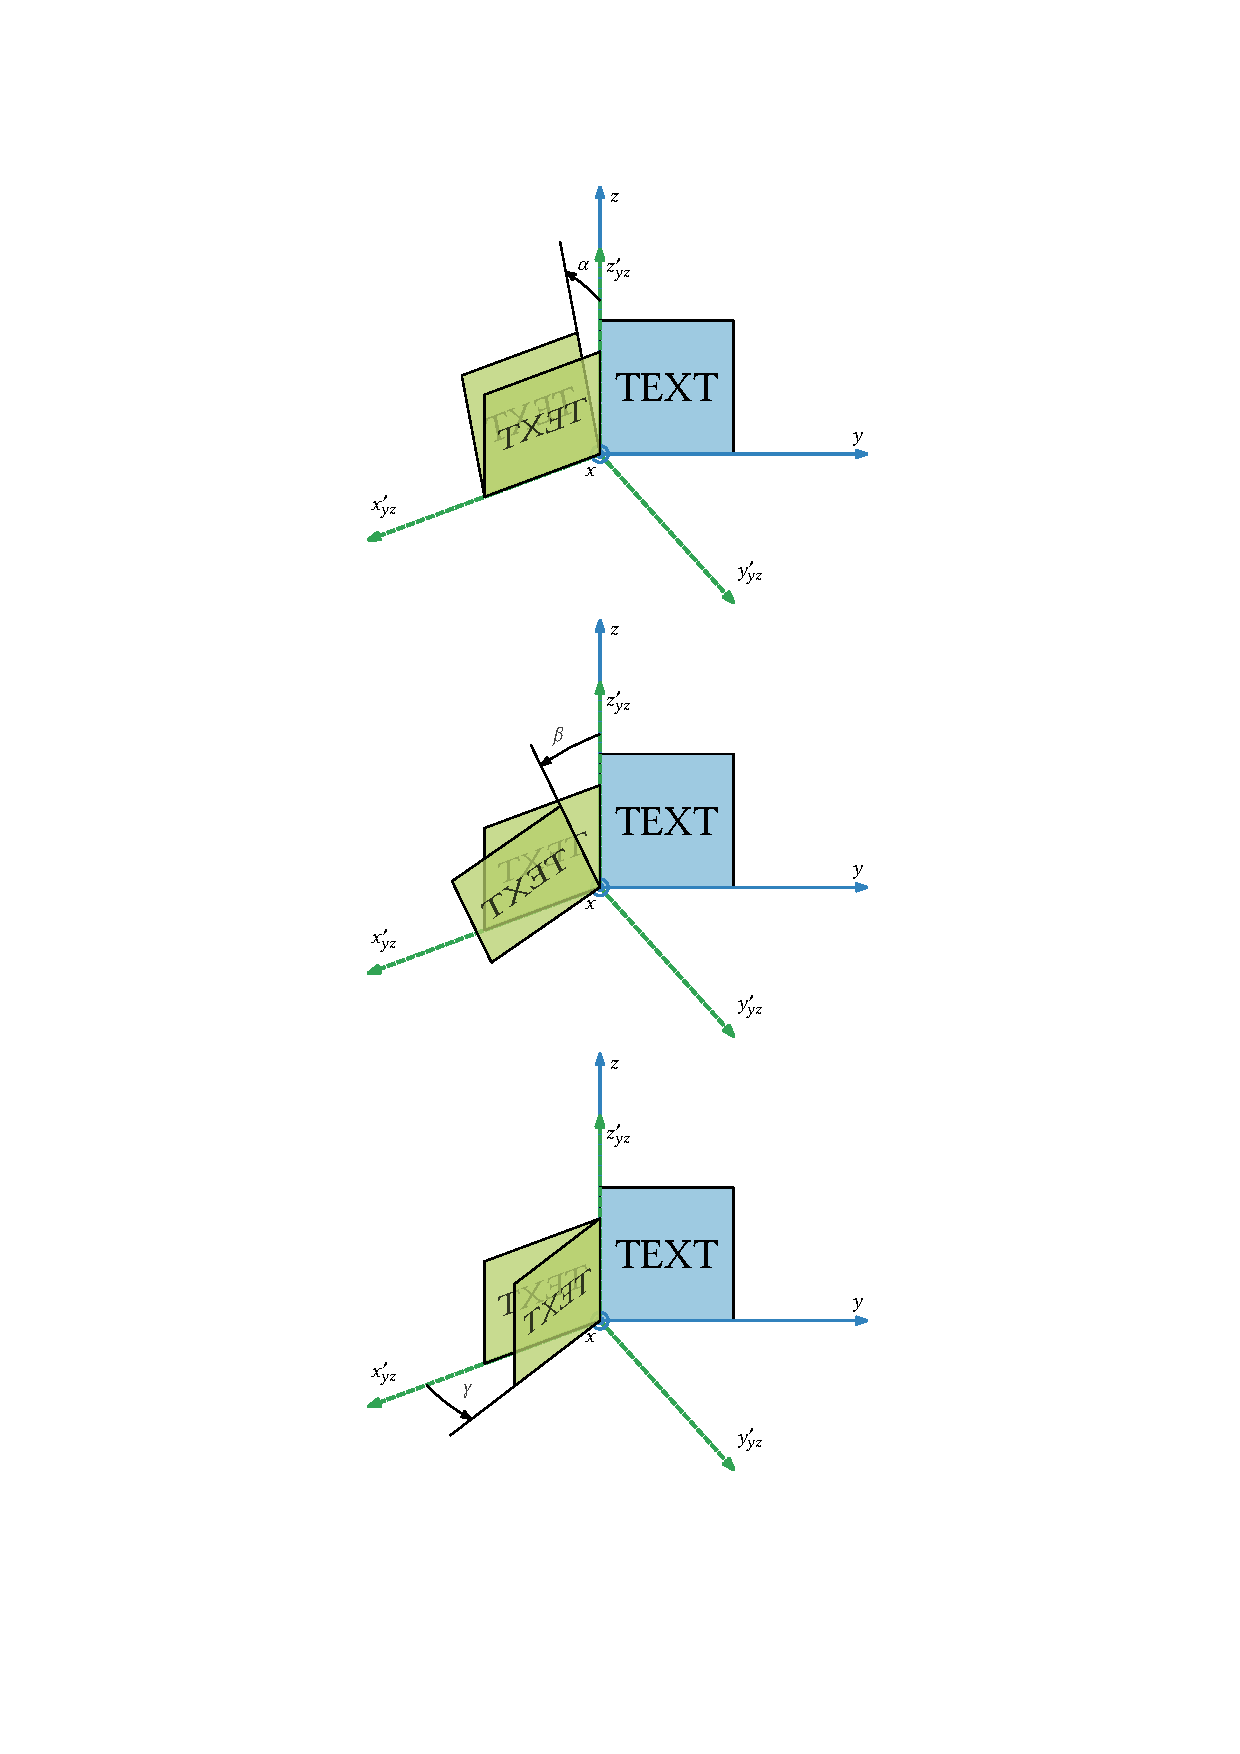
\includegraphics[scale=1]{pdf/projection_explained_extra_rot_xz_v2.pdf}
%\caption{Extra rotation for projection onto the $xz$ plane.}
%\label{fig:extra_rot_2xz}
%\end{center}
%\end{figure}

%\begin{figure}
%\begin{center}
%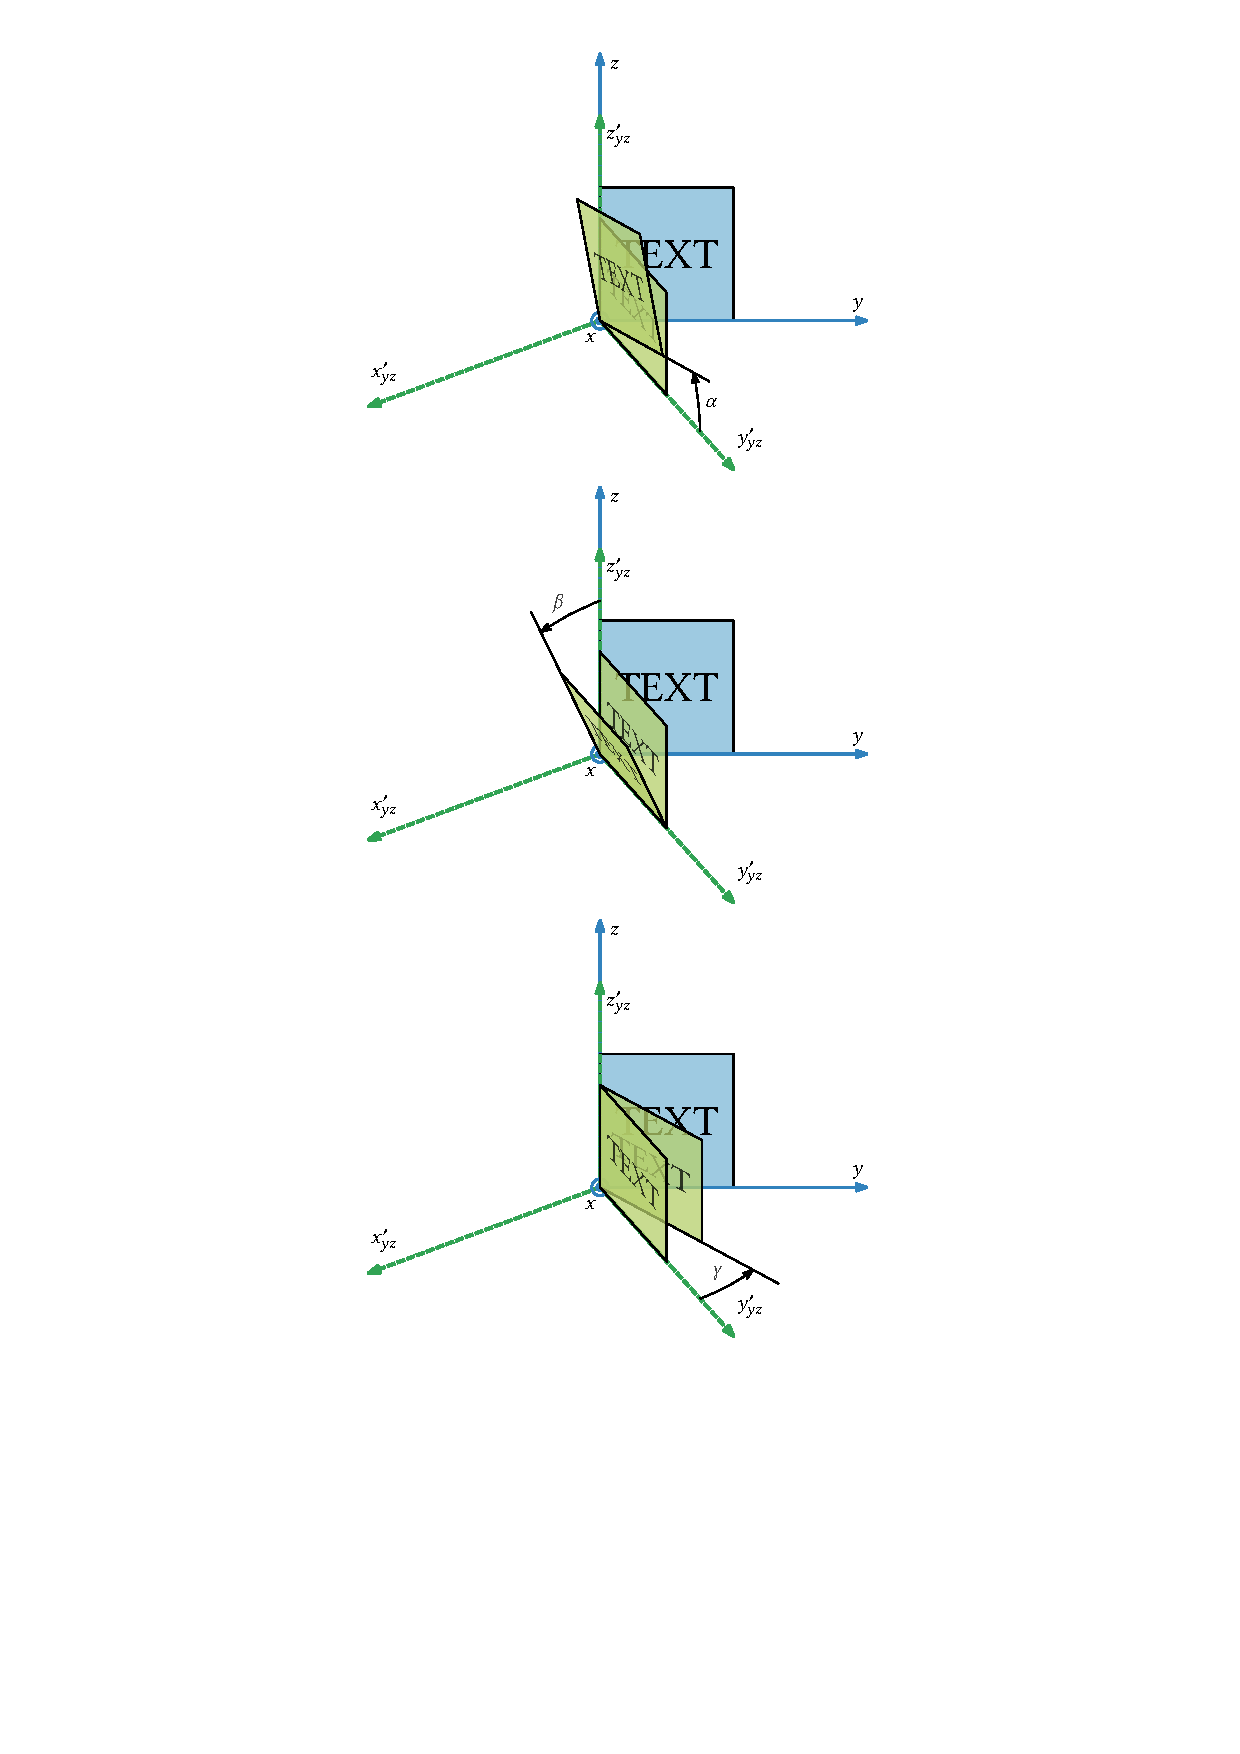
\includegraphics[scale=1]{pdf/projection_explained_extra_rot_yz_v2.pdf}
%\caption{Extra rotations for projection onto the $yz$ plane.}
%\label{fig:extra_rot_3yz}
%\end{center}
%\end{figure}

\clearpage
\section*{Appendix B: Examples of use}
\addcontentsline{toc}{section}{Appendix B: Examples of use}

A few examples are presented below to illustrate some possible use of this ipelet.

\subsection{Electromagnetic wave}

\begin{center}
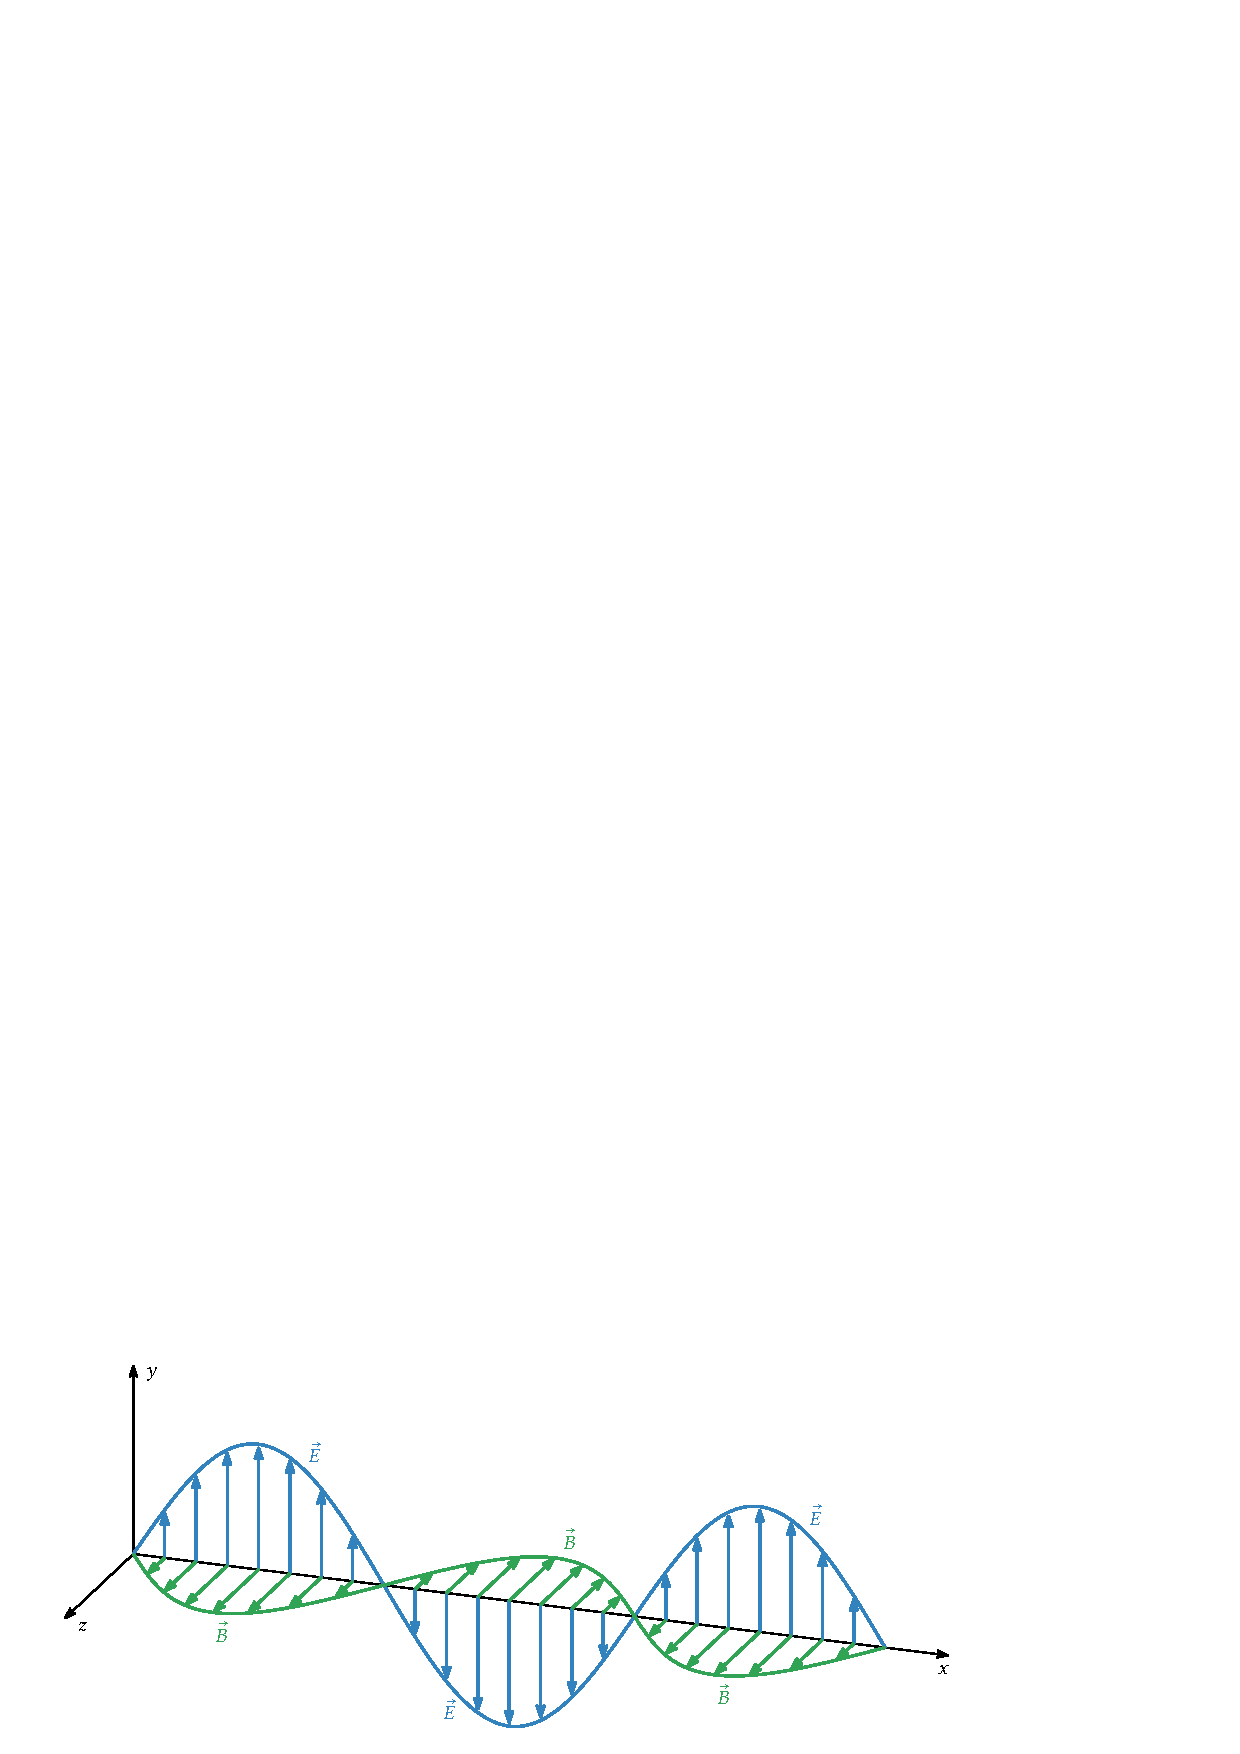
\includegraphics[scale=1]{pdf/examples/elmag_wave_1.pdf}
\end{center}

\subsection{Optical abberation}

\begin{center}
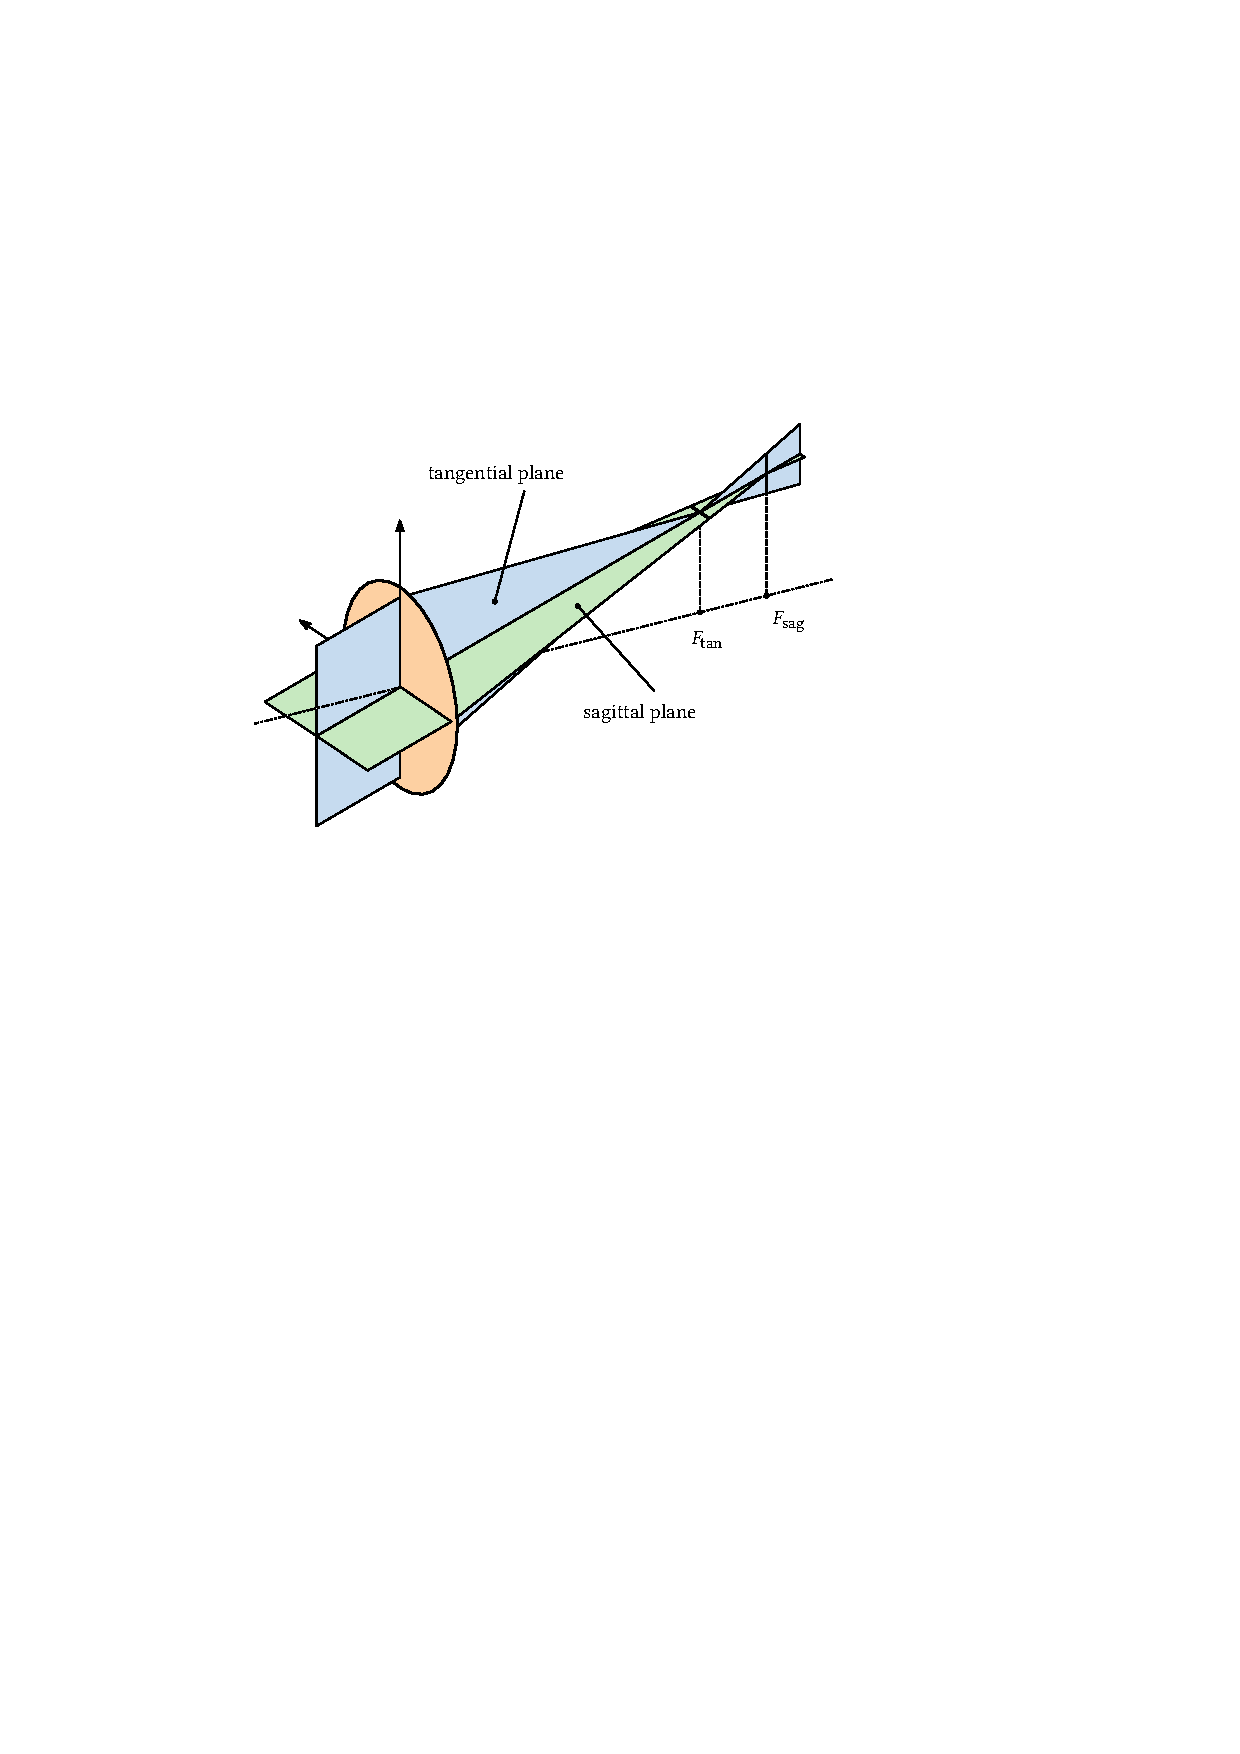
\includegraphics[scale=1]{pdf/examples/astigmatismus.pdf}
\end{center}

%\subsection{Reciprocal space}

% or crystal lattice (maybe reciprocal...)

\subsection{Cylindrical coordinates}

\begin{center}
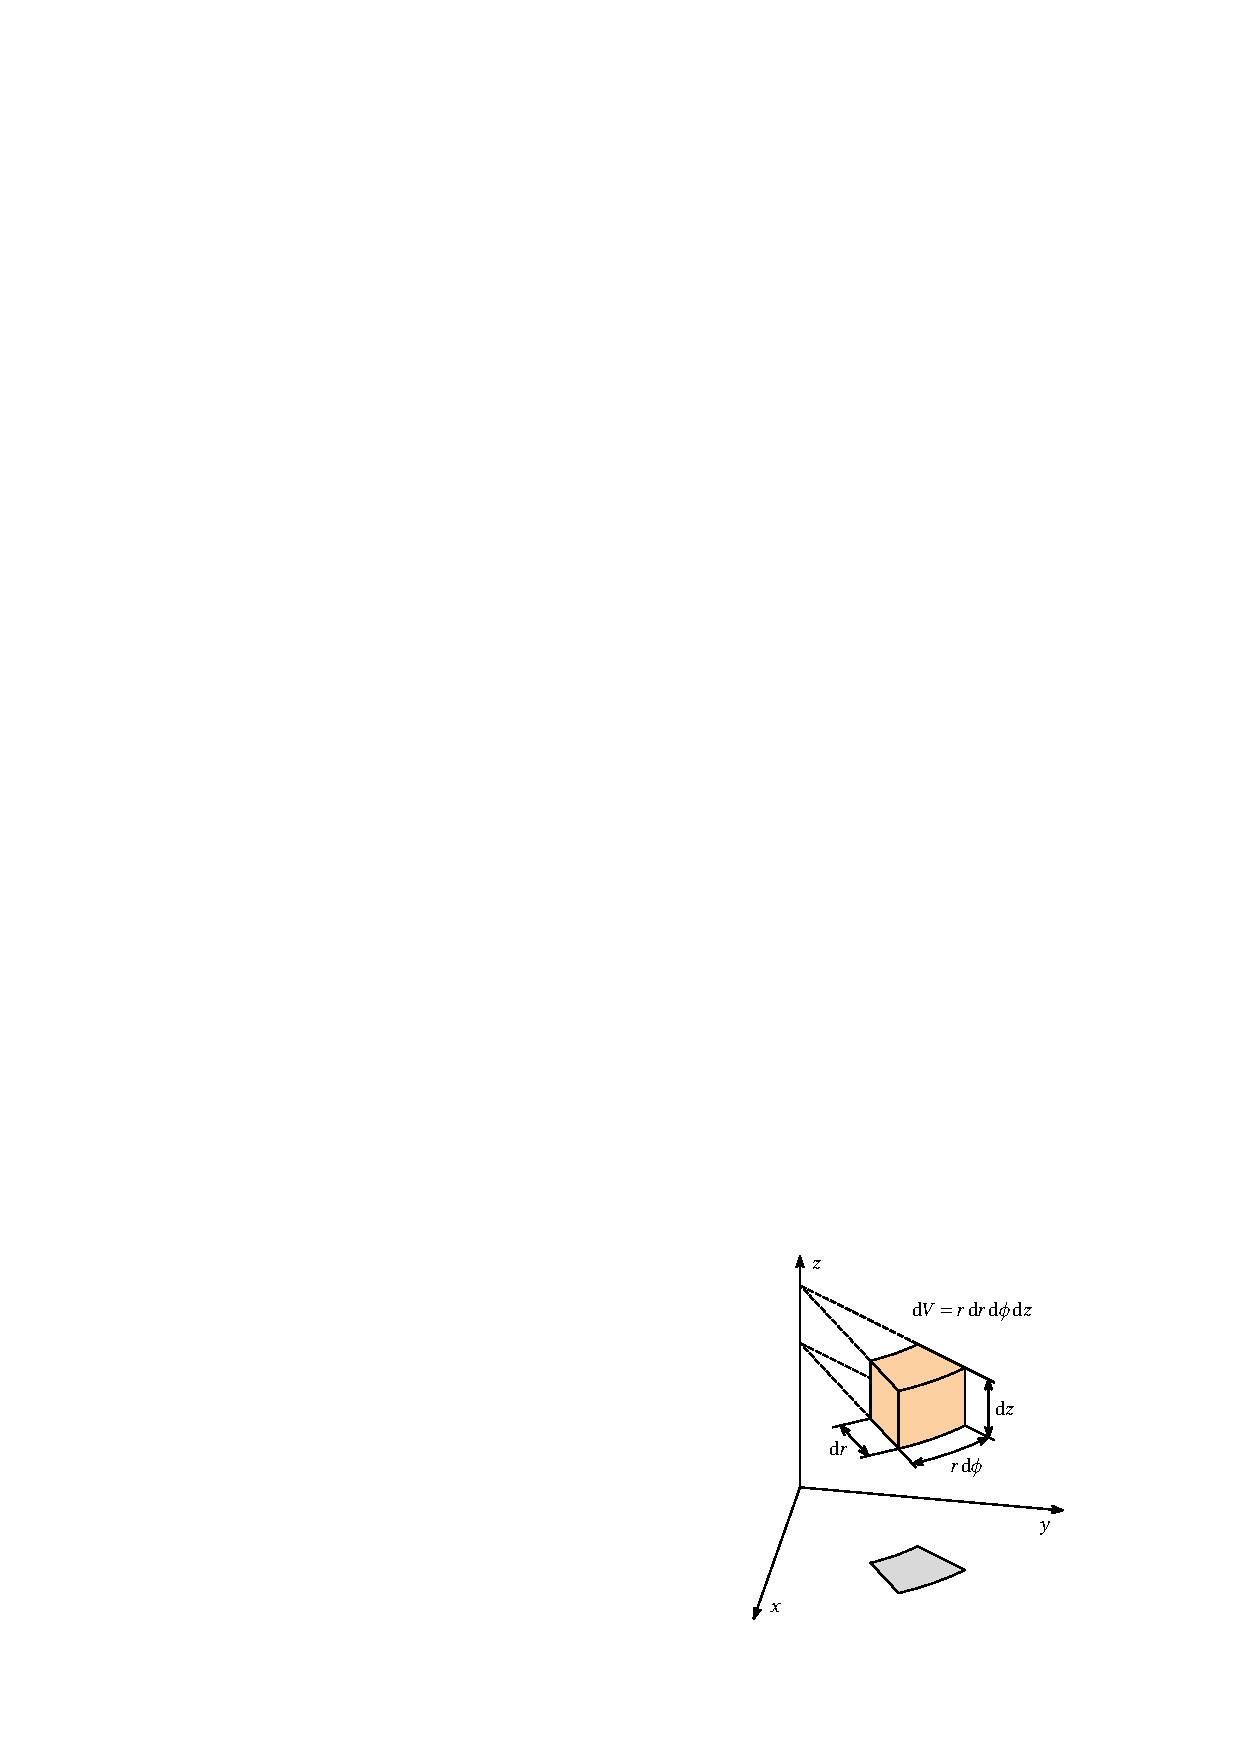
\includegraphics[scale=1]{pdf/examples/diff_element_cyl_coord_1.pdf}
\end{center}


\end{document}